\documentclass{book}
\usepackage{fancyhdr, graphicx, multicol}

\title{\huge \textbf{The Hog Programming Language}}
\author{Jason Halpern \\ jrh2170 \\ Testing/Validation
        \and Samuel Messing \\ sbm2158 \\ Project Manager
        \and Benjamin Rapaport \\ bar2150 \\ System Architect
        \and Kurry Tran \\ klt2127 \\ System Integrator
        \and Paul Tylkin \\ pt2302 \\ Language Guru}

\begin{document}
\maketitle

\tableofcontents

\chapter{Introduction}
\label{chap:intro}

\section{Taming the Elephant}
\label{sec:elephant}

As data sets have grown in size, so have the complexities of dealing with them.
For instance, consider wanting to generate counts for all the words in War and
Peace by means of distributed computation. Writing in Java and using Hadoop
MapReduce (TM),\footnote{\texttt{http://hadoop.apache.org/}} a simple solution
takes over 50 lines of code, as the programmer is required to specify
intermediate objects not directly related to the desired computation, but
required simply to get Hadoop to function properly. Our goal is to produce a
language that can express the same computation in about 10 lines.

Hog is a \textbf{data-oriented}, high-level, scripting language for creating
MapReduce\cite{dean:2004} programs. Used alongside Hadoop, Hog enables users to
efficiently carry out \textbf{distributed} computation. Hadoop MapReduce is an
open-source framework for carrying out distributed computation, which is
especially useful for working with large data sets. While it is possible to
write code to carry out computations with Hadoop directly, the framework
requires users to specify low-level details that are often irrelevant to their
desired goal. 


By building a scripting language on top of Hadoop, we aim to simplify the
process. Built around a \textbf{simple} and highly \textbf{readable} syntax,
Hog will let users focus on \emph{what} computations they want done, and not
\emph{how} they want to do them.  Hog takes care of all the low-level details
required to run computations on Hadoop’s distributed network. All a user needs
to do is tell Hog the location of their valid Hadoop instance, and Hog will do
the rest.

\subsection{Data-Oriented}
\label{sub:data-oriented}

Hog is a powerful language that allows for the efficient handling of
structured, unstructured and semi-structured data. Specifically, Hog simplifies
the process of writing programs to handle the distributed processing of
data-intensive applications. Programmers using Hog only have to express the
steps for processing the data in the Map and Reduce functions without having to
be concerned with relations and the constraints imposed by a traditional
database schema. Hog also provides control flow structures to manipulate this
data. In addition, Hog frees a programmer from having to write each step in a
data processing task since many of those low-level processing details are
handled by the language and the system.

Hog uses Hadoop MapReduce (TM), an open-source MapReduce framework written in
Java. Hadoop’s run time system takes care of the details of partitioning the
input data, scheduling the program’s execution across machines, counteracting
machine failures, and managing inter-machine communication. Hadoop also
distributes data to machines and tries to collocate chunks of data with the
nodes that need it, therefore maximizing data locality and giving good
performance.


\subsection{Simple}
\label{sub:simple}

To write a simple word count program in Java using the Hadoop framework
requires over 59 lines of
code.\footnote{\texttt{http://hadoop.apache.org/common/docs/current/mapred\_tutorial.html}}
The same program written in Hog requires just 10 lines. The discrepancy comes
from the fact that Hog takes care of the low-level details required to
correctly communicate and interact with the Hadoop framework. This allows users
to enhance the expressive potential of their programs, without sacrificing
power. All that Hog requires a user to do is specify the location of their
valid Hadoop instance, write a map function to process a segment of data, write
a reduce function to combine the results, and Hog takes care of the rest.


\subsection{Distributed}
\label{sub:distributed}

As datasets have exploded in size, programmers have had to deal with the
challenge of writing programs for distributed systems that process data in a
time-efficient manner. One of the benefits of using Hadoop is that it allows
programmers to write parallel programs without needing to understand the
intricacies of how the distributed computations are implemented. This benefit
is one of the key reasons for the widespread adoption of Hadoop. Since Hog
operates as a layer on top of Hadoop, and abstracts away even more of the
implementation details of the distributed system, we remain committed to the
ideal of a fully distributed language that is easy for programmers to use. Once
again, this is paramount to Hog’s focus on what computations are being done and
not how they are being done.

\subsection{Readable}
\label{sub:readable}

The syntax of Hog is designed to make programs as readable as possible. Hog is
specifically developed to make simple calculations easy to carry out. While Hog
may not be the best solution for highly sophisticated analysis, an individual
desiring to learn more about Hadoop and the MapReduce technique will find Hog
an inviting environment to get started. Hog’s syntax is simple enough that
someone with only a small amount of programming experience should have no
trouble understanding the basics of what is happening in a sample Hog program.
Our goal is to let users think about their data first and foremost, and not on
using or learning an esoteric syntax. Where possible, our syntax decisions
prefer simplicity over complexity.

\subsection{A Sample Program}
\label{sub:sample}

\begin{verbatim}
1  @Map (int lineNum, text line) -> (text, int) {
2    # for every word on this line, emit that word and the number 1
3    foreach text word in line.tokenize(" ") {
4       emit(word, 1); } 
5  }

6  @Reduce (text word, iter<int> values) -> (text, int) {
7    # initialize count to zero
8    int count = 0;
9    while( values.hasNext() ) {
10     # for every instance of '1' for this word, add to count.
11     count = count + values.next(); }
12   # emit the count for this particular word
13   emit(word, count);
14 }

15 @Main {
16   # call map reduce
17   mapReduce();
18 }
\end{verbatim}

This program generates a count of the number of instances of every word in a
file. Here is the first 50 lines of output generated by \tt WordCount.hog \rm
called on the full text of \emph{War and
Peace}\footnote{\texttt{http://www.gutenberg.org/ebooks/2600/} was used as the
input text}:

\begin{verbatim}
31784	the
21049	and
16389	to
14895	of
10056	a
8314	in
7847	he
7645	his
7425	that
7255	was
5540	with
5316	had
4492	not
4209	at
4162	her
4009	I
3757	it
3744	as
3495	on
3488	him
3308	for
3134	is
2888	but
2762	The
2718	you
2636	said
2620	she
2526	from
2390	all
2387	were
2354	be
2333	by
2031	who
2006	which
1910	have
1812	He
1777	one
1727	they
1693	this
1645	what
1566	or
1561	an
1554	Prince
1550	so
1541	Pierre
1466	been
1439	did
1424	up
1409	their
1342	woul
\end{verbatim}



\chapter{Tutorial}
\label{chap:tutor}

Use your updated tutorial.

\chapter{Language Reference Manual}
\label{chap:LRM}

\section{Introduction}
\label{sec:introduction}

As data sets have grown in size, so have the complexities of dealing with them.
For instance, consider wanting to generate counts for all the words in \emph{War
and Peace} by means of distributed computation. Writing in Java and using Hadoop
MapReduce (TM), a simple solution takes over 50 lines of code, as the programmer
is required to specify intermediate objects not directly related to the desired
computation, but required simply to get Hadoop to function properly. Our language 
can express the same computation in about 15 lines.

\subsection{The MapReduce Framework}
\label{sub:mapreduce}

With the explosion in the size of datasets that companies have had to manage in
recent years, there are many new challenges that they face. Many companies and
organizations have to handle the processing of datasets that are terabytes or even
petabytes in size. The first challenge in this large-scale processing is how to
make sense of all this data. More importantly, the question is how they can 
process and manipulate the data in a time-efficient and reliable manner. 
The second challenge is how they handle this across their distributed systems. Writing distributed, fault-tolerant programs requires a high level of expertise and knowledge of parallel systems.

In response to this need, a group of engineers at Google developed the MapReduce
framework in 2004. This high-level framework can be used for a variety of
tasks, including handling search queries, indexing crawled documents, and
processing logs. The software framework was developed to handle computations on
massive datasets that are distributed across hundreds or even thousands of
machines. The motivation behind MapReduce was to create a unified framework that
abstracted away many of the low level details from programmers, so they would not
have to be concerned with how the data is distributed, how the computation is
parallelized and how all of this is done in a fault tolerant manner.

The MapReduce framework partitions input data across different machines, so
that the computations are initially performed on smaller sets of data
distributed across the cluster. Each cluster has a master node that is
responsible for coordinating the efforts among the slave nodes. Each slave node
sends periodic heartbeats to the master node so it can be aware of progress and
failure. In the case of failure, the master node can reassign tasks to other
nodes in the cluster. In conjunction with the underlying MapReduce framework
created at Google, the company also had to build the distributed Google File
System (GFS). This file system ``allows programs to access files efficiently
from any computer, so functions can be mapped
everywhere.''\cite{patterson:2008} GFS was designed with the same goals as
other distributed file systems, including ``performance, scalability,
reliability and availability.''\cite{ghemawat:2003} Another key aspect of the
GFS design is fault tolerance and this is achieved by treating failures as
normal and optimizing for ``huge files that are mostly appended to and then
read.''\cite{ghemawat:2003}

Within the framework, a programmer is responsible for writing both map and
reduce functions. The map function is applied to all of the input data ``in
order to compute a set of intermediate key/value pairs.''\cite{dean:2004} In
the map step, the master node partitions the input data into smaller problems
and distributes them across the worker nodes in the cluster. This step is
applied in parallel to all of the input that has been partitioned across the
cluster. Then, the reduce step is responsible for collecting all the processed
data from the slave nodes and formatting the output. The reduce function is
carried out over all the values that have the same key such that each key has a
single value. which is the answer to the problem MapReduce is trying to solve.
The output is done to files in the distributed file system.

The use of ``a functional model with user-specified map and reduce operations
allows (Google) to parallelize large computations easily and to use
re-execution as the primary mechanism for fault tolerance.''\cite{dean:2004} A
programmer only has to specify the functions described above and the system
handles the rest of the details. Figure \ref{fig:map_reduce_overview}
illustrates the execution flow of a MapReduce program.

\begin{center}
\begin{figure}
  \label{fig:map_reduce_overview}
  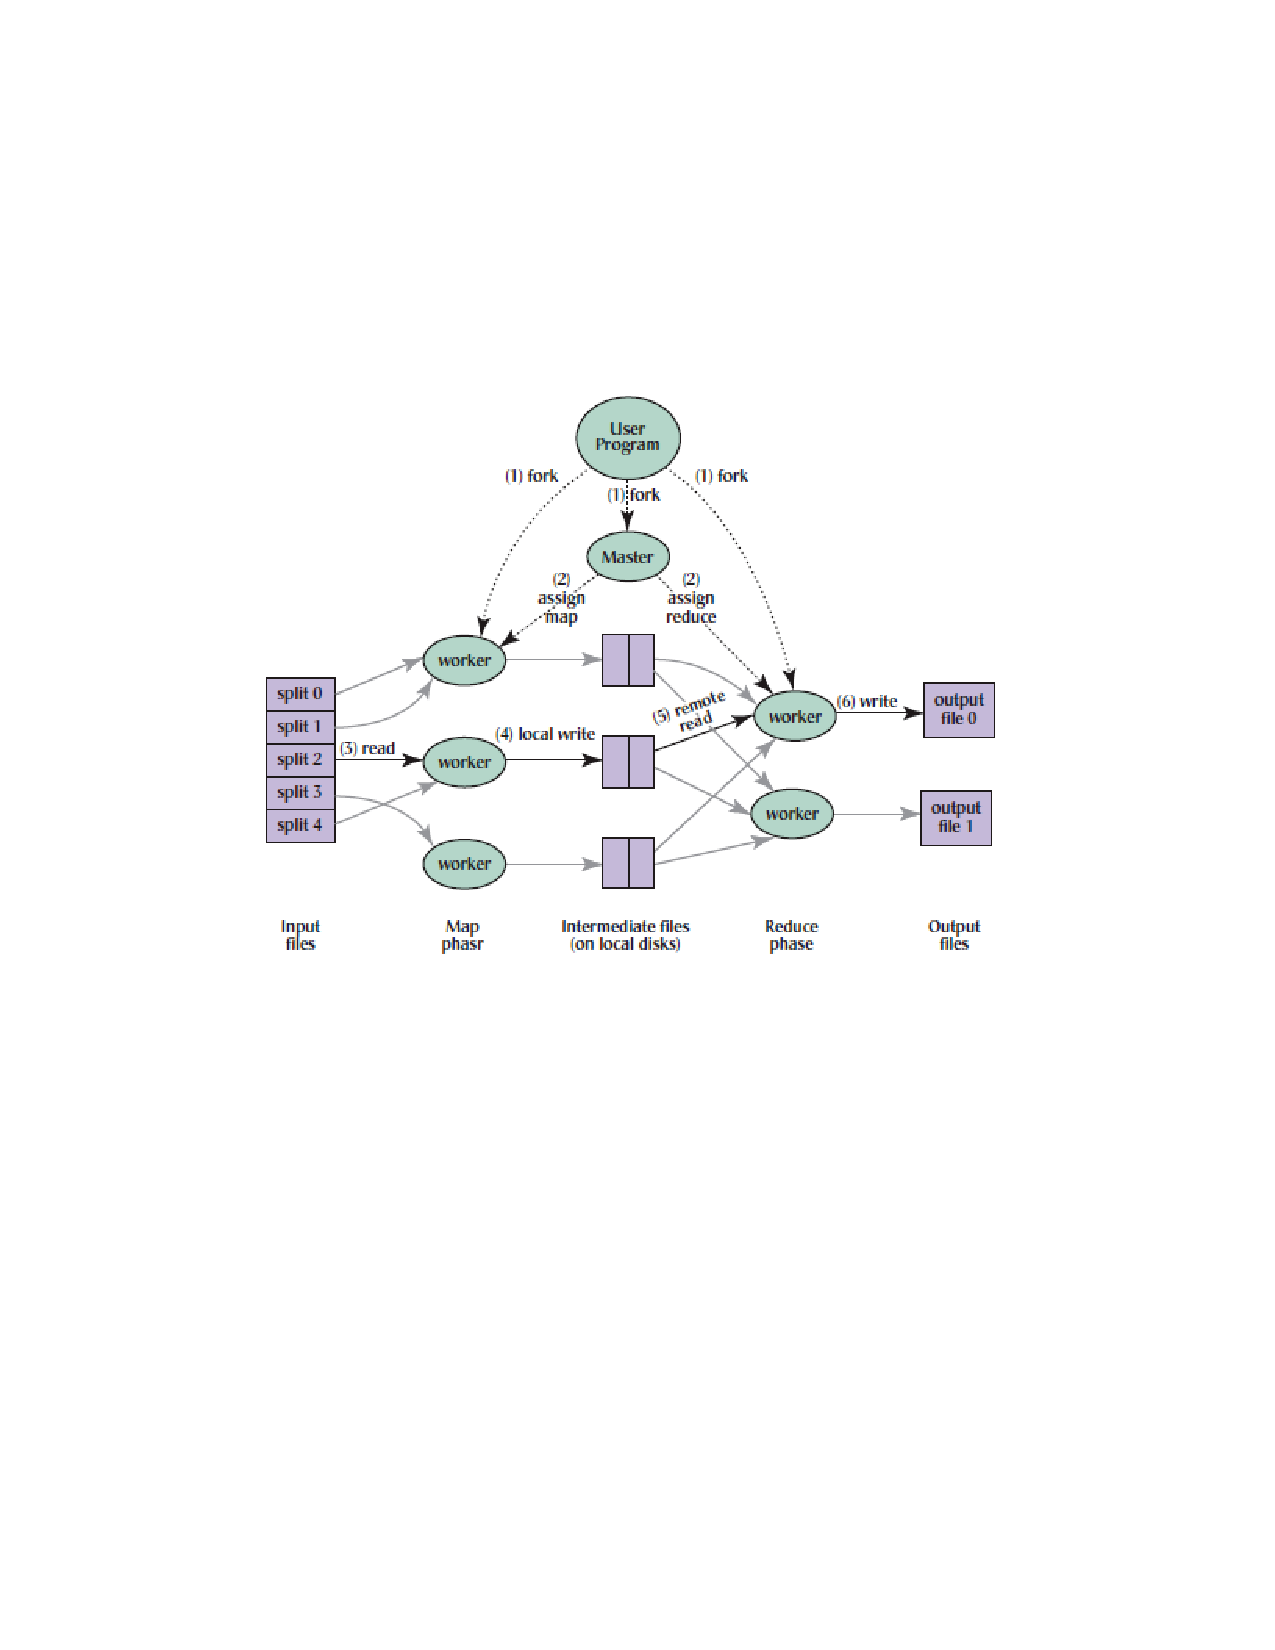
\includegraphics[width=1.0\textwidth]{img/map_reduce_overview.pdf}
  \caption{Overview of the MapReduce program, from \cite{ghemawat:2003}.}
\end{figure}
\end{center}

\subsection{The Hog Language}
\label{sub:hog_language}

Hog is a \textbf{data-oriented}, \textbf{high-level}, scripting language for
creating MapReduce programs. Used alongside Hadoop, Hog enables users to
efficiently carry out \textbf{distributed} computation. Hadoop MapReduce is an
open-source implementation of the MapReduce framework, which is especially useful
for working with large data sets. While it is possible to write code to carry out
computations with Hadoop directly, the framework requires users to specify
low-level details that are often irrelevant to their desired goal.

By building a scripting language on top of Hadoop, we aim to simplify the process.
Built around a \textbf{simple} and highly \textbf{readable} syntax, Hog will let
users focus on what computations they want done, and not how they want to do them.
Hog takes care of all the low-level details required to run computations on
Hadoop’s distributed network. All a user needs to do is tell Hog the location of
their valid Hadoop instance, and Hog will do the rest.

We intentionally have restricted the scope of Hog to deal with specific
problems.  For example, Hog only supports reading and writing plaintext files.
While these limitations sacrifice the generality of the language, they promote
ease of use.

\subsubsection{Guiding Principles} % (fold)
\label{ssub:guiding_principles}

The guiding principles of Hog are:

\begin{itemize}
  \item Anyone can MapReduce
  \item Brevity over verbosity
  \item Simplicity over complexity
\end{itemize}


% subsubsection guiding_princples (end)

\subsection{The ``Ideal'' Hog User} % (fold)
\label{sub:the_ideal_hog_user}

Hog was designed with a particular user in mind: one that has already learned
the basics of programming in a different programming language (such as Java or
Python), but is inexperienced with distributed computation and can benefit from
a highly structured framework for writing MapReduce programs. The language was
designed with the goal of making learning how to write MapReduce programs as
easy as possible. However, the user should be adept with programming concepts
such as program structure, control flow (iteration and conditional operators),
evaluation of boolean expressions, etc.

% subsection the_ideal_hog_user (end)


\section{Syntax Notation} % (fold)
\label{sec:syntax_notation}

In the syntax notation used throughout the Hog manual, different syntactic
categories are noted by \emph{italic type}, and literal words and characters
are in \tt typewriter style\rm. When specific terms are introduced,
\textbf{\emph{emboldened, italicized font}} is used.

% sec syntax_notation (end)

\section{Program Structure} % (fold)
\label{sec:program_structure}

\subsection{Overall Structure} % (fold)
\label{sub:overall_structure}

Every Hog program consists of a single source file with a ‘.hog’ extension. This
source file must contain three sections: \tt @Map\rm, and \tt @Reduce\rm, and
\tt @Main \rm and can also include an optional \tt @Functions \rm section. These
sections must be included in the following order:

\begin{verbatim}
   @Functions {
      .
      .
      .
    }
    @Map <type signature> {
      .
      .
      .
    }
    @Reduce <type signature> {
      .
      .
      .
    }
    @Main {
      .
      .
      .
    }
\end{verbatim}

% section overall_structure (end)

\subsection{\tt @Functions\rm} % (fold)
\label{sub:tt_functionsrm}

At the top of every Hog program, the programmer has the option to define functions
in a section called \tt @Functions\rm. Any function defined in this section can be
called from any other section of the program, including \tt @Map\rm, \tt
@Reduce\rm, and \tt @Main \rm and can also be called from other functions defined
in the \tt @Functions \rm section. The section containing the functions begins
with the keyword \tt @Functions \rm on its own line, followed by the function
definitions.

Function definitions have the form:

\begin{quotation}
  \emph{type functionName} \tt ( \rm \emph{parameterList} \tt ) \{ \rm \\
  \indent \indent \emph{expressionList}; \\
  \indent \tt \}
\end{quotation}

where,

\begin{quotation} \emph{parameterList} $\rightarrow$ \emph{parameter} \tt , \rm
\emph{parameterList} $|$ \emph{parameter} \end{quotation}

The return type can be any valid Hog type. The rules regarding legal function
names are identical to those regarding legal variable identifiers. Each
parameter in the parameter list consists of a valid Hog type followed by the
name of the parameter, which must also follow the naming rules for identifiers.
Parameters in the parameter list are separated by commas. The \tt @Functions
\rm section ends when the next Hog section begins.

A complete example of an \tt @Functions \rm section:

\begin{verbatim}
    @Functions {
      int min(int a, int b) {
        if (a < b) {
          return a;
        } else {
          return b;
        }
      }

      list<int> reverseList(list<int> oldList) {
        list<int> newList;
        for (int i = oldList.size() - 1; i >= 0; i--;) {
          newList.add(oldList.get(i));
        }
        return newList;
      }
    }
\end{verbatim}

User-defined functions can make reference to other user-defined functions.
However, function names cannot be overloaded (i.e. it is not possible to use
the same function name with a parameter list that differs in the number of
arguments or argument types). Disallowing function overloading is a design
choice consistent with Hog's guiding principle of simplicity.

% section tt_functionsrm (end)

\subsection{\tt @Map \rm} % (fold)
\label{sub:tt_map_rm}

The map function in a MapReduce program takes as input key-value pairs, performs
the appropriate calculations and procedures, and emits intermediate key-value
pairs as output. Any given input pair may map to zero, one, or multiple output
pairs. The \tt @Map \rm section defines the code for the map function.

The \tt @Map \rm header must be followed by the signature of the map function, and
then the body of the map function as follows:

\begin{quotation} \tt @Map ( \rm \emph{type identifier, type identifier} \tt )
-> ( \rm \emph{type, type} \tt ) \{ \\ \indent \indent . \\ \indent \indent .
\\ \indent \indent . \\ \indent \tt \} \rm \end{quotation}

The first \emph{type identifier} defines the \emph{\textbf{key}} and the second
defines the \emph{\textbf{value}} of the input key-value pair to the \tt @Map
\rm function. The identifiers specified for the key and value can be made
reference to later within the \tt @Map \rm block. The \tt @Map \rm signature is
followed by an arrow and another key-value pair, defining the types of the
output of the map function. Notice that identifiers are not specified for the
output key and value (said to be \emph{\textbf{unnamed}}), as these pairs are
only produced at the end of the map function. 

The map function can include any number of calls to \tt emit()\rm, which outputs
the resulting intermediate key-value pairs for use by the function defined in the
\tt @Reduce \rm section. The types of the values passed to the \tt emit() \rm
function must agree with the signature of the output key-value pair as defined in
the \tt @Map \rm type signature. All output pairs from the map function are
subsequently grouped by key by the framework, and passed as input to the \tt
@Reduce \rm function.

\emph{Note}: In the current version of the language, the only configuration
available is for a file to be passed into the map function one line at a time,
with the line of text being the value, and the corresponding line number as the
key. This requires that the input key/value pair to the map function is of type
\tt (int key‐name, text value‐name)\rm. Extending this to allow for other input
formats is a future goal of the Hog language.

The following is an example of a complete \tt @Map \rm section for a program that
counts the number of times each word appears in a set of files. The map function
receives a single line of text, and for each word in the line (as delineated by
whitespace), it emits the word as the key with a value of one. By emitting the word
as the key, we can allow the framework to group by the word, thus calling the
reduce function for every word.

\begin{verbatim}

  @Map (int lineNum, text line) -> (text, int) {
      # for every word on this line, emit that word and the number 1
      foreach text word in line.tokenize(" ") {
          emit(word, 1);
       }
   }

\end{verbatim}


% section tt_map_rm (end)

\subsection{\tt @Reduce \rm} % (fold)
\label{sub:tt_reduce_rm}

The reduce function in a MapReduce program takes a list of values that share the
same key, as emitted by the map function, and outputs a smaller set of values to
be associated with another key. The input and output keys do not have to match,
though they often do.

The setup for the reduce section is similar to the map section. However, the input
value for any reduce function is always an iterator over the list of values
associated with its key. The type of the key must be the same as the type of the
key emitted by the map function. The iterator must be an iterator over the type of
the values emitted by the map function.

\begin{quotation}
  \tt @Reduce ( \rm \emph{type identifier, type identifier} \tt ) -> ( \rm \emph{type, type} \tt ) \{ \\
  \indent \indent . \\
  \indent \indent . \\
  \indent \indent . \\
  \indent \tt \} \rm
\end{quotation}

As with the map function, the reduce function can emit as many key/value pairs as
the user would like. Any key/value pair emitted by the reduce function is recorded
in the output file.

Below is a sample \tt @Reduce \rm section, which continues the word count example,
and follows the \tt @Map \rm sample introduced in the previous section.

\begin{verbatim} 

    @Reduce (text word, iter<int> values) -> (text, int) {
      # initialize count to zero
      int count = 0;
      while (values.hasNext()) {
        # for every instance of '1' for this word, add to count
        count = count + values.next();
      }
      # emit the count for this particular word
      emit(word, count);
    }

\end{verbatim} 

% subsection tt_reduce_rm (end)

\subsection{\tt @Main \rm} % (fold)
\label{sec:tt_main_rm}

The \tt @Main \rm section defines the code that is the entry point to a Hog
program. In order to run the MapReduce program defined by the user in the
previous sections, \tt @Main \rm must contain a call to the system-level
built-in function \tt mapReduce() \rm, which calls the \tt @Map \rm and \tt
@Reduce \rm functions. Other arbitrary code can be run from the \tt @Main \rm
section as well. In the current version of the language, \tt @Main \rm does not
have access to the results of the MapReduce program resulting from a call to
\tt mapReduce()\rm. Therefore, it is quite common for the \tt @Main \rm section
to contain the call to \tt mapReduce() \rm and nothing else.

Below is a sample \tt @Main \rm section which prints to the standard output and
runs a map reduce job.

\begin{verbatim}
    @Main {
          print("Starting mapReduce job.\n");
          mapReduce();
          print("mapReduce complete.\n");
    }
\end{verbatim}


% subsection tt_main_rm (end)

% section program_structure (end)

\section{Lexical Conventions} % (fold)
\label{sec:lexical_conventions}

\subsection{Tokens} % (fold)
\label{sub:tokens}

The classes of tokens include the following: identifiers, keywords,
constants, string literals, operators, and separators. Blanks, tabs, newlines, and
comments are ignored. If the input is separated into tokens up to a given
character, the next token is the longest string of characters that could represent
a token.

% subsection tokens (end)

\subsection{Comments} % (fold)
\label{sub:comments}

Multi-line comments are identified by the enclosing character sequences \tt
\#\{ \rm and \tt \}\#\rm. Anything within these enclosing characters is
considered a comment, and is completely ignored by the compiler. For example,

\begin{verbatim}
    int i = 0;
    #{ these are block
        comments and are ignored
         by the compiler }#
    i++;

\end{verbatim}

In the above example, the text \tt these are block comments \textbackslash n
comments and are ignored \textbackslash n by the complier \rm is completely
ignored during compilation. Compilation goes directly from the line \tt int i =
0; \rm to the line \tt i++;\rm.

Single-line comments are defined to be strings of text included between a '\tt
\#\rm' symbol on the left-hand side and a newline character ('\tt\textbackslash
n\rm') on the right-hand side.

% subsection comments (end)

\subsection{Identifiers} % (fold)
\label{sub:identifiers}

A valid identifier in Hog is a sequence of contiguous letters, digits, or
underscores, which are used to distinguish declared entities, such as methods,
parameters, or variables from one another. A valid identifier also provide a
means of determining scope of an entity, and helps to determine whether the
same valid identifier in another scope refers to the same entity. The first
character of an identifier must not be a digit. Valid identifiers are case
sensitive, so \tt foo \rm is not the same identifier as \tt Foo\rm.

% section identifiers (end)

\subsection{Keywords} % (fold)
\label{sub:keywords}

The following words are reserved for use as keywords, and may not be redefined
by the programmer:

\begin{multicols}{4}
\tt
\begin{itemize}
 
  \item[] add
  \item[] and
  \item[] bool
  \item[] break
  \item[] catch
  \item[] clear
  \item[] contains
  \item[] containsAll
  \item[] continue
  \item[] default
  \item[] else
  \item[] elseif
  \item[] emit
  \item[] final
  \item[] for
  \item[] foreach
  \item[] Functions
  \item[] get
  \item[] hadoop
  \item[] hasNext
  \item[] if
  \item[] in
  \item[] instanceof
  \item[] int
  \item[] int2real
  \item[] int2text
  \item[] isEmpty
  \item[] iter
  \item[] list
  \item[] Map
  \item[] mapReduce
  \item[] next
  \item[] not
  \item[] or
  \item[] peek
  \item[] print
  \item[] real
  \item[] real2int
  \item[] real2text
  \item[] Reduce
  \item[] remove
  \item[] removeAll
  \item[] return
  \item[] size
  \item[] sort
  \item[] text
  \item[] text2int
  \item[] text2real
  \item[] throw
  \item[] tokenize
  \item[] try
  \item[] void
  \item[] while
  
  
\end{itemize}
\rm
\end{multicols}

% subsection keywords (end)

\subsection{Constants} % (fold)
\label{sub:constants}

The word \textbf{\emph{constant}} has two different meanings in Hog. It can
refer to either a variable that is \emph{fixed}, that is, once it is
initialized cannot be changed, or can refer to an \textbf{\emph{unnamed
value}}, such as "1.0". To declare a constant variable, use the following
pattern,

\begin{quotation}
   \tt final \rm \emph{type variableName} = \emph{value};
\end{quotation}

The following are a list of examples of unnamed values and their corresponding
types:

\begin{itemize}
  \item[] \tt -1\rm, \tt 0\rm, \tt 1\rm, \tt 2\rm $\hfill$ (all of type \tt int\rm)
  \item[] \tt -0.12\rm, \tt3.14159\rm, \tt 2.7182\rm, \tt 1.41421 \rm $\hfill$ (all of type \tt real\rm)
  \item[] \tt true\rm, \tt false \rm $\hfill$ (all of type \tt bool\rm)
\end{itemize}

% subsection constants (end)

\subsection{Text Literals} % (fold) \label{sub:string_literals} 

A text literal consists of a sequence of zero of more contiguous characters
enclosed in double quotes, such as \tt "hello"\rm. A text literal can also
contain escape characters such as \tt "\textbackslash n" \rm for the new line
character or \tt "\textbackslash t" \rm for the tab character. A text literal
has many of the same built-in functions as the String class in Java. String
literals are constant and their values cannot be changed after they are
created. String literals can be concatenated with adjacent text literals by use
of the \tt + \rm operator and are then converted into a single \tt text \rm
variable. Hog implements concatenation by use of the Java \tt StringBuilder \rm
(or \tt StringBuffer\rm) class and its append method. All text literals in Hog
programs are implemented as instances of the \tt text \rm class, and then are
mapped directly to the equivalent \tt String \rm class in
Java.\footnote{Technically, \tt text \rm objects are implemented as instances
of Hadoop's \tt Text \rm class, which is closely related to the Java \tt String
\rm class.}

% subsection string_literals (end)

\subsection{Variable Scope} % (fold)
\label{sub:variable_scope}

Hog implements what is generally referred to as lexical scoping or block scope. An
identifier is valid within its enclosing block. The identifier is also valid for
any block nested within its enclosing block.

% subsection variable_scope (end)


\subsection{Argument Passing}
\label{sub:argument_passing}

Since Hog is compiled into Java, it passes arguments using call-by-value.
However, similarly to Java, it is possible to imitate call-by-reference
behavior. 

\subsection{Evaluation Order}
\label{sub:evaluation_order}

Hog uses applicative order (eager) evaluation, similarly to Java.

% section lexical_conventions (end)


\section{Types} % (fold)
\label{sec:types}

\subsection{Basic Types} % (fold)
\label{sub:basic_types}

The basic types of Hog include \tt int \rm (integer numbers in base 10, 64
bytes in size), \tt real \rm (floating point numbers, 64 bytes in size), \tt
bool \rm(boolean values, \tt true \rm or \tt false \rm) and \tt text \rm
(Strings, variable in size).  Unlike some languages, Hog includes no basic
character type. Instead, a programmer makes use of \tt text\rm s of size 1.

\emph{Implementation details}: Hog’s primitive types are not so primitive. They are
in fact wrappers around Hadoop classes. For instance, Hog’s \tt int \rm type is a
wrapper around Hadoop's \tt IntWritableclass\rm. The following lists for every
primitive type in Hog the corresponding Hadoop class that the type is built on top
of:

\begin{center}
\begin{tabular}{|c|c|}
    \hline
\textbf{Hog Type} & \textbf{Enclosed Hadoop Class} \\ \hline
\tt int & \tt IntWritable \\ \hline
\tt real & \tt DoubleWritable \\ \hline
\t bool & \tt BooleanWrtiable \\ \hline
\tt text & \tt Text \rm \\ \hline
\end{tabular}
\end{center}

% subsection basic_types (end)

\subsection{Derived Types (Collections)} % (fold)
\label{sub:derived_types_collections_}

There are two derived types that can be created by the programmer: \tt
list<T>\rm and \tt set<T>\rm.  Future versions of Hog are expected to implement
other derived types, including dictionaries/hash maps, user-defined iterators,
and multisets. The \tt list<T> \rm type is an ordered collection of objects of
the same type. The \tt set<T> \rm is an unordered collection of unique objects
of the same type. Hog supports arbitrarily nested derived types, so it is
possible, for example, to have a \tt list\rm  of \tt list\rm s of \tt list\rm s
of \tt int\rm s.

A special derived type is \tt iter<T>\rm, which is Hog's iterator object. An
\tt iter \rm object is associated with a list, and allows one traversal of the
elements in the list; this is used by Hog in the \tt @Reduce \rm section of a
Hog program.

% subsection derived_types_collections_ (end)

\subsection{Type Conversions} % (fold)
\label{sub:conversions}

\textbf In order to cast a variable to be of a different type, use the
following notation:

\begin{quotation}
      \tt \emph{primitiveType}(2\emph{otherPrimitiveType})\rm \emph{variableName}
\end{quotation}

Hog supports casting between the primitive types \tt int\rm, \tt real\rm, and
\tt text\rm, via the built-in functions \tt int2real\rm, \tt int2text\rm, \tt
real2int\rm, \tt real2text\rm, \tt text2int\rm, and \tt text2real\rm. If
casting a text to an int or real results in an invalid number (e.g. \tt
text2int("1a4") \rm), a run-time exception will be thrown.

% subsection conversions (end)

% section types (end)

\section{Expressions} % (fold)
\label{sec:expressions}

\subsection{Operators} % (fold)
\label{sub:operators}

\subsubsection{Arithmetic Operators} % (fold)
\label{ssub:arithmetic_operators}

Hog implements all of the standard arithmetic operators. All arithmetic
operators are only defined for use between variables of numeric type (\tt
int\rm, \tt real\rm) with the exception that the \tt + \rm operator is also
defined for use between two \tt text \rm variables. In such instances, \tt +
\rm is defined as concatenation. Thus, in the following,

\begin{verbatim}
    text face = "face";
    text book = "book";
    text facebook = face + book;
\end{verbatim}

After execution, the variable \tt facebook \rm will have the value
``facebook''. No other arithmetic operators are defined for use with \tt text
\rm variables, and \tt + \rm is only valid if both variables are of type \tt
text \rm. Otherwise, the program will result in a compile-time \tt
TypeMismatchException\rm. 

When an arithmetic operator is used between two numeric variables of different
type, as in,

\begin{verbatim}
    int a = 1;
    real b = 2.0;
\end{verbatim}

\noindent the non-\tt real \rm variable would first need to be cast into a \tt
real \rm before operating on them, so that both operands have the
same type. So thus

\begin{verbatim}
   print(a + b);
\end{verbatim}

would throw an error, while

\begin{verbatim}
   print(int2real(a) + b);
\end{verbatim}

would print 3.0.

If one of the operands happens to have a \tt null \rm value (for instance, if a
variable is \textbf{\emph{uninitialized}}), then the resulting operation will
cause a run-time \tt NullValueException\rm, and the program will crash.

\begin{center}
\begin{tabular}{|c|c|c|c|c|}

\hline \textbf{Operator} & \textbf{Arity} & \textbf{Associativity} &
\textbf{Precedence Level} & \textbf{Behavior} \\ \hline
\tt + \rm & binary & left & 0 & addition \\ \hline
\tt - \rm & binary & left & 0 & minus \\ \hline
\tt * \rm & binary & left & 1 & multiplication \\ \hline
\tt / \rm & binary & left & 1 & division \\ \hline
\tt \% \rm & binary & left & 2 & mod$\dagger$
\\ 
\hline
\tt ++ \rm & unary & left & 3 & increment \\ \hline
\tt -- \rm & unary & left & 3 & decrement \\ \hline
\tt - \rm & unary & right & 3 & negate \\ \hline
\end{tabular}
\end{center}

$\dagger$Follows Java's behavior: a modulus of a negative number is a negative
number.
% subsubsection arithmetic_operators (end)

\subsubsection{Logical Operators} % (fold)
\label{ssub:logical_operators}

The following are the logical operators implemented in Hog. Note that these
operators only work with two operands of type \tt bool\rm. Attempting to use a
logical operator with an object of any other type results in a compile-time
exception (see \S \ref{sub:compile_time_exceptions}).

\begin{center}
\begin{tabular}{|c|c|c|c|c|}

\hline \textbf{Operator} & \textbf{Arity} & \textbf{Associativity} &
\textbf{Precedence Level} & \textbf{Behavior} \\ \hline
\tt or \rm & binary & left & 0 & logical or \\ \hline
\tt and \rm & binary & left & 1 & logical and \\ \hline
\tt not \rm & unary & right & 2 & negation \\ \hline
\end{tabular}
\end{center}

% subsubsection logical_operators (end)

\subsubsection{Comparators} % (fold)
\label{ssub:comparators}

The following are the comparators implemented in Hog (all are binary operations).

\begin{center}
\begin{tabular}{|c|c|c|c|}

\hline \textbf{Operator} & \textbf{Associativity} &
\textbf{Precedence Level} & \textbf{Behavior} \\ \hline
\tt < \rm & none & 0 & less than \\ \hline
\tt <= \rm & none & 0 & less than or equal to \\ \hline
\tt > \rm & none & 0 & greater than \\ \hline
\tt >= \rm & none & 0 & greater than or equal to \\ \hline
\tt == \rm & none & 0 & equal \\ \hline
\tt != \rm & none & 0 & not equal \\ \hline

\end{tabular}
\end{center}

\emph{Note}: All comparators do not work with non-numeric or non-boolean types.
Comparisons require that the two operands be either both numeric or both
boolean, and a numeric value cannot be compared to a boolean value. If the two
operands are numeric but of different types, one of them must be cast so that
they are of the same type. The only valid comparators that can be used with
boolean expressions are \tt == \rm and \tt !=\rm. The use of a comparison
operator in Hog between any two derived types will result in a run-time error.

% subsubsection comparators (end)

\subsubsection{Assignment} % (fold)
\label{ssub:assignment}

There is one assignment operator, '\tt =\rm'. Expressions involving the
assignment operator have the following form:

\begin{quotation}
\emph{identifier}$_1$ \tt = \rm \emph{expression} $|$ \emph{identifier}$_2$
\end{quotation}

At compile time, the compiler checks that both the result of the \emph{expression}
(or \emph{identifier}$_2$) and \emph{identifier}$_1$ have the same type. If not, a
compile-time \tt TypeMismatchException \rm will be thrown.

% subsubsection assignment (end)

% subsection operators (end)

% section expressions (end)

\section{Declarations} % (fold)
\label{sec:declarations}

A user is only allowed to use variables/functions after they have been
declared. When declaring a variable, a user must include both a type and an
identifier for that variable. Otherwise, an exception will be thrown at compile
time.

\subsection{Type Specifiers} % (fold)
\label{sub:type_specifiers}

Every variable, whether its type is primitive or derived, must be assigned a
type upon declaration, for instance,

\begin{verbatim}
    list<int> myList;
\end{verbatim}

declares the variable \tt myList \rm to be a \tt list \rm of \tt int\rm s,

\begin{verbatim}
    list<list<int>> myOtherList;
\end{verbatim}

declares the variable \tt myOtherList \rm to be a \tt list \rm of \tt list\rm s
of \tt int \rm s,

and

\begin{verbatim}
    text myText;
\end{verbatim}

declares the variable \tt myText \rm to be of type \tt text\rm .

% subsection type_specifiers (end)

\subsection{Declarations} % (fold)
\label{sub:declarations}

\subsubsection{Null Declarations} % (fold)
\label{ssub:null_declarations}

If a variable is declared but not initialized, the variable becomes a
\textbf{\emph{null reference}}, which means it points to nothing and holds no
data (internally, this means that an entry has been added to Hog's symbol table
with that variable name).

% subsubsection null_declarations (end)

\subsubsection{Primitive-Type Variable Declarations} % (fold)
\label{ssub:primitive_type_variable_declarations}

Variables of one of the primitive types, including \tt int\rm, \tt real\rm, \tt
text\rm, or \tt bool\rm, are declared using the following patterns:

\begin{enumerate}
  \item \emph{type identifier} \rm $\hfill$ (uninitialized)
  \item \emph{type identifier = expression } \rm $\hfill$ (initialized)
\end{enumerate}

When the first pattern is used, we say that the variable is
\textbf{\emph{uninitialized}}, and has the value \tt null\rm. When the second
pattern is used, we say that the variable is \textbf{\emph{initialized}}, and has
the same value as the value of the result of the \emph{expression}. The
\emph{expression} must return a value of the right type, or the compiler will
throw a \tt TypeMismatchError\rm. The \emph{expression} may contain an expression
involving both other variables and unnamed raw primitives (e.g. 1 or 2), an
expression involving only other variables or unnamed raw primitives, or a single
variable, or a single unnamed raw primitive.

% subsubsection primitive_type_variable_declarations (end)

\subsubsection{Derived-Type Variable Declarations} % (fold)
\label{ssub:derived_type_variable_declarations}

Derived-type variables are declared using the following pattern:

\begin{enumerate}
  \item \emph{type identifier;}
\end{enumerate}

When the derived type is first declared, we say that the variable is
\textbf{\emph{uninitialized}}, and has the value \tt null\rm. If a user
attempts to use any type-­specific operations that are not meaningful (for
instance, \tt myList.size() \rm on an uninitialized variable, the program will
throw a run­time exception (see \S \ref{sec:exception_handling} for a
discussion of exceptions)). The example code below initializes a \tt list\rm of
integers and adds one element to it.

\begin{verbatim}
    list<int> myList;
    myList.add(5);
\end{verbatim}

% subsubsection derived_type_variable_declarations (end)

\subsubsection{Function Declarations} % (fold)
\label{ssub:function_declarations}

In order to declare a function, use the following notation:

\begin{quotation}
\emph{type functionName} \tt ( \rm \emph{parameterList} \tt ) \{ \rm \\
\indent \indent \emph{expressionList} \\
\indent \tt \}
\end{quotation}


% subsubsection function_declarations (end)

% subsection declarations (end)

% section declarations (end)

\section{Statements} % (fold)
\label{sec:statements}

\subsection{Expression Statement} % (fold)
\label{sub:expression_statement}

An \textbf{\emph{expression statement}} is either an individual assignment or a
function call. All consequences of a given expression take effect before the next
expression is executed.

% subsection expression_statement (end)

\subsection{Compound Statement (Blocks)} % (fold)
\label{sub:compound_statement}

\textbf{\emph{Compound statements}} are defined by \{ and \} and are used to
group a sequence of statements, so that they are syntactically equivalent to a
single statement.

% subsection compound_statement (end)

\subsection{Flow-Of-Control Statements} % (fold)
\label{sub:flow_of_control_statements}

The following are the \textbf{\emph{flow-of-control}} statements included in Hog:

\begin{itemize}
  \item[] \tt if ( \rm \emph{expression} \tt ) \rm \emph{statement}
  \item[] \tt if ( \rm \emph{expression} \tt ) \rm \emph{statement} \tt else \rm \emph{statement}
  \item[] \tt if ( \rm \emph{expression} \tt ) \rm \emph{statement} \tt elseif ( \rm \emph{statement} \tt ) $\dots$ else 
  \rm \emph{statement}
\end{itemize}

In the above statements, the  $\dots$ signifies an unlimited number of \tt
elseif \rm statements, since there is no limit on the number of \tt elseif \rm
statements that can appear before the final \tt else \rm statement. In the
second statement above, when the expression in the \tt if \rm statement
evaluates to \tt false\rm, then the \tt else \rm statement will execute. In the
third statement above with \tt if\rm, \tt elseif \rm and \tt else \rm
statements, the statement will be executed that follows the first expression
evaluating to \tt true\rm. If none of these expressions evaluate to \tt
true\rm, then the \tt else \rm statement is executed.

To increase the expressive power of Hog, flow-of-control statements can also be
nested within each other.

% subsection flow_of_control_statements (end)

\subsection{Iteration Statements} % (fold)
\label{sub:iteration_statements}

Iteration statements signify looping and can appear in one of the two following
forms:

\begin{itemize}
  \item[] \tt while ( \rm \emph{expression} \tt ) \rm \emph{statement}
  \item[] \tt for ( \rm \emph{expression}$_1$ \tt ; \rm \emph{expression}$_2$ \tt ; \rm \emph{expression}$_3$ \tt ;) \rm \emph{statement}
  \item[] \tt foreach \rm \emph{expression} \tt in \rm \emph{iterable-object statement}
\end{itemize}

In the \tt while \rm pattern, the associated \emph{statements} will be executed
repeatedly until the \emph{expression} evaluates to \tt false\rm. The
\emph{expression} is evaluated before every iteration. Please note that in a
slight syntactical departure from Java, Hog requires a semicolon after the
third expression (the increment step) in the \tt for\rm loop construct. Thus,
an example of correct Hog syntax would be \begin{verbatim} for (int i = 0; i <
10; i++;){...}\end{verbatim}

In the \tt for \rm pattern, \emph{expression}$_1$ is the initialization step,
\emph{expression}$_2$ is the test or condition and \emph{expression}$_3$ is the
increment step. At each step through the for loop, \emph{expression}$_2$ is
evaluated. When \emph{expression}$_2$ evaluates to false, iteration through the
loop ends.

In the \tt foreach \rm pattern, the iteration starts at the first element in the
\emph{iterable-object statement} (a statement that evaluates to an object that
supports the \tt iterator() \rm function). The \emph{statement} executes during
every iteration. The iteration ends when the \emph{statement} has been executed
for each item in the iterable object and there are no items left to iterate
through.

\subsubsection{Example of \tt while \rm} % (fold)
\label{ssub:example_1}

\begin{verbatim}
    int i = 0;
    while (i < 10) {
      print(i);
      i++;
    }

\end{verbatim}

% subsubsection example_1 (end)

\subsubsection{Example of \tt for \rm} % (fold)
\label{ssub:example_2}

\begin{verbatim}
    for (int i = 0; i < 10; i++;) {
      print(i)
    }
\end{verbatim}

% subsubsection example_2 (end)

\subsubsection{Example of \tt foreach \rm} % (fold)
\label{ssub:example_3}

\begin{verbatim}
    # we first initialize and populate the list as follows: 
    list<int> iList;
    for (int i = 0; i < 10; i++;) {
       iList.add(i);
    }

    # This is an example of using foreach
    # Note that the type of the iterable must be declared.    

    foreach int i in iList {
      print(i);
    }
\end{verbatim}

% subsubsection example_3 (end)

% subsection iteration_statements (end)

% section statements (end)

\section{Built-in Functions} % (fold)
\label{sec:built_in_functions}

Hog includes both \emph{\textbf{system-level}} and \emph{\textbf{object-level}}
built-in functions. Here \emph{\textbf{built-in}} means functions provided by the
language itself.

\subsection{System-level Built-ins} % (fold)
\label{sub:system_level_built_ins}

Hog includes a number of system­level built­in functions that can be called from
various sections of a Hog program. The functions are:

\begin{itemize} 

\item[] \tt void emit(key, value) \rm \\

This function can be called from the \tt @Map \rm and \tt @Reduce \rm sections in
order to communicate the results of the map and reduce functions to the Hadoop
platform. The types of the key/value pairs must match those defined as the output
types in the header of each section.

\item[] \tt void mapReduce() \rm \\

This function can be called from the \tt @Main \rm section in order to initiate
the mapreduce job, as definied in the \tt @Map \rm and \tt @Reduce \rm sections.
Any Hog program that implements mapreduce will need to call this function in \tt
@Main\rm.

\item[] \tt void print(toPrint) \rm \\

This function can be called from the \tt @Main \rm section in order to print to
standard output. The argument must be a primitive type.

\end{itemize}

% subsection system_level_built_ins (end)

\subsection{Object-level Built-ins} % (fold)
\label{sub:object_level_built_ins}

The derived type objects have several built-in functions that provide
additional functionality. All of these functions are invoked using the
following pattern:

\begin{quotation}
\emph{identifier.functionName(parameterList)}
\end{quotation}

\noindent Where \emph{identifier} is the identifier for the object in question,
\emph{functionName} is the name of the function, and \emph{parameterList} is a
(possibly empty) list of parameters used to specify the behavior of the
invocation.

\emph{Note}: In what follows, if a function has return type T, it means that
the return type of this function matches the parameterized type of this object
(i.e. for an \tt iter<int> \rm object, these functions have return type \tt
int\rm).

\subsubsection{\tt iter \rm} % (fold)
\label{ssub:iter}

\tt iter \rm is Hog's iteration object, and supports several built-in functions
that are independent of the particular type of the \tt iter \rm object. The
built-in functions are as follows:

\begin{itemize}

\item[] \tt bool hasNext() \rm

This function returns \tt true \rm if the iterator object has a next object
to return, and \tt false \rm otherwise.

\item[] \tt T next() \rm

This function returns the next object (if one exists) for the owning \tt iter \rm
object. A call to \tt next() \rm differs from a call to \tt peek() \rm in that the
function call advances the cursor of the iterator.

\item[] \tt T peek() \rm

This function returns the next object (if one exists) for the owning \tt iter
\rm object. A call to \tt peek() \rm returns the object without advancing the
iterator's cursor, thus multiple calls to \tt peek() \rm without any
intermediate function calls will all return the same value.

\end{itemize} 


% subsubsection iter (end)

\subsubsection{\tt list \rm} % (fold)
\label{ssub:list}

\begin{itemize}

\item[] \tt void add(T itemToAdd) \rm

Adds the object passed to the end of the list. The object must be of the same
type as the list, or the operation will result in a \textbf{compile-time or
run-time} exception.

\item[] \tt void clear() \rm

Removes all elements in this \tt list\rm.

\item[] \tt T get(int index) \rm

Returns the item from the list at the specified index.


\item[] \tt void sort() \rm

Function that sorts the items in the list in lexicographical ascending order.

\item[] \tt int size() \rm

Returns an int with the number of elements in the list.

\end{itemize}


% subsubsection list (end)

\subsubsection{\tt set \rm} % (fold)
\label{ssub:tt_set_rm}

\begin{itemize}

\item[] \tt bool add(T element) \rm

Returns \tt true \rm if the element was successfully added to the \tt set\rm, \tt false \rm otherwise.

\item[] \tt void clear() \rm

Removes all elements from the \tt set \rm such that it is empty afterwards.

\item[] \tt bool contains(T element) \rm

Returns \tt true \rm if the \tt set \rm contains this element, \tt false \rm otherwise.

\item[] \tt bool containsAll(set<T> otherSet) \rm

Returns \tt true \rm if all elements in \tt otherSet \rm are found in this set.

\item[] \tt bool isEmpty() \rm

Returns \tt true \rm if there are no elements in this \tt set\rm, \tt false \rm otherwise.

\item[] \tt iter<T> iterator() \rm

Returns an iterator over the elements in this \tt set\rm.

\item[] \tt bool remove(T element) \rm

Returns \tt true \rm if the element was successfully removed from the \tt set\rm, \tt false \rm otherwise (i.e. the \tt list
\rm didn't contain \tt element\rm).

\item[] \tt bool removeAll(set<T> otherSet) \rm

Returns \tt true \rm if all the elements in \tt otherSet \rm were successfully removed from this set.

\item[] \tt int size() \rm

Returns the number of elements in the set.

\end{itemize}

% subsubsection tt_set_rm (end)

\subsubsection{text} % (fold)
\label{ssub:text}

The following function can be called on a \tt text \rm object:

\begin{itemize}

\item[] \tt int length() \rm \\

Returns the length (number of individual characters) of this \tt text\rm.

\item[] \tt text replace(text matchText, text replacementText) \rm \\

Returns a new \tt text \rm object with each sub-\tt text \rm that matches \tt
matchText \rm replaced by \tt replacementText\rm. This function does \textbf{not}
alter the original \tt text \rm object.

\item[] \tt list<text> tokenize(text delimiter) \rm \\

\tt tokenize() \rm can be called on a \tt text \rm object to tokenize it into a
list of \tt text \rm objects based on the delimiter. The delimiter is not included
in any of the \tt text \rm objects in the returned list.

\end{itemize}

% subsubsection text (end)

% subsection object_level_built_ins (end)

% section built_in_functions (end)

\section{System Configuration} % (fold)
\label{sec:system_configuration}

The user must set configuration variables in the \tt hog.rb \rm build script to
allow the Hog compiler to link the Hog program with the necessary jar files to run
the MapReduce job. The user must also specify the job name within the Hog source
file.

\begin{itemize}

\item[] \textbf{HADOOP\_HOME} absolute path of hadoop folder
\item[] \textbf{HADOOP\_VERSION} hadoop version number
\item[] \textbf{JAVA\_HOME} absolute path of java executable
\item[] \textbf{JAVAC\_HOME} absolute path of javac executable
\item[] \textbf{HOST} where to job is rsynced to and run
\item[] \textbf{LOCALMEM} how much memory for java to use when running in local mode 
\item[] \textbf{REDUCERS} the number of reduce tasks to run, set to zero for map only jobs

\end{itemize}

% section system_configuration (end)

\section{Compilation Structure} % (fold)
\label{sec:parsing_tools}

Currently, the Hog compiler is implemented as a translator into the Java
programming language. The first phase of Hog compilation uses the JFlex as its
lexical analyzer, which is designed to work with the Look-Ahead Left-to-Right
(LALR) parser generator CUP. The lexical analyzer creates lexemes, which are
logically meaningful sequences, and for each lexeme the lexical analyzer sends
to the LALR parser a token of the form \tt $<$token-name,
attribute-value$>$\rm. The second phase of Hog compilation uses Java CUP to
create a syntax tree, which is a tree-like intermediate representation of the
source program, which depicts the grammatical structure of the Hog source
program.

In the last phase of compilation, the Hog semantic analyzer generates Java source
code, which is then compiled into byte code by the Java compiler. Then with the
Hadoop Java Archives (JARs) the bytecode is executed on the Java Virtual Machine
(JVM). With the syntax tree and the information from the symbol table, the Hog
compiler then checks the Hog source program to ensure semantic consistency with
the language specification. The syntax tree is initially untyped, but after
semantic analysis Hog types are added to the syntax tree. Hog types are
represented in two ways, either a translation of a Hog type into a new Java class,
or by mapping Hog types to the equivalent Java types. Mapping Hog types directly
to Java types improves performance because a JVM can handle primitive types much
more efficiently than objects. Also, a JVM implements optimizations for well-known
types, such as String, and thus Hog is built for optimal performance.

% section parsing_tools (end)

\section{Linkage and I/O} % (fold)
\label{sec:linkage_and_i_o}

\begin{center}
\begin{figure}
  \label{fig:hog_compiler}
  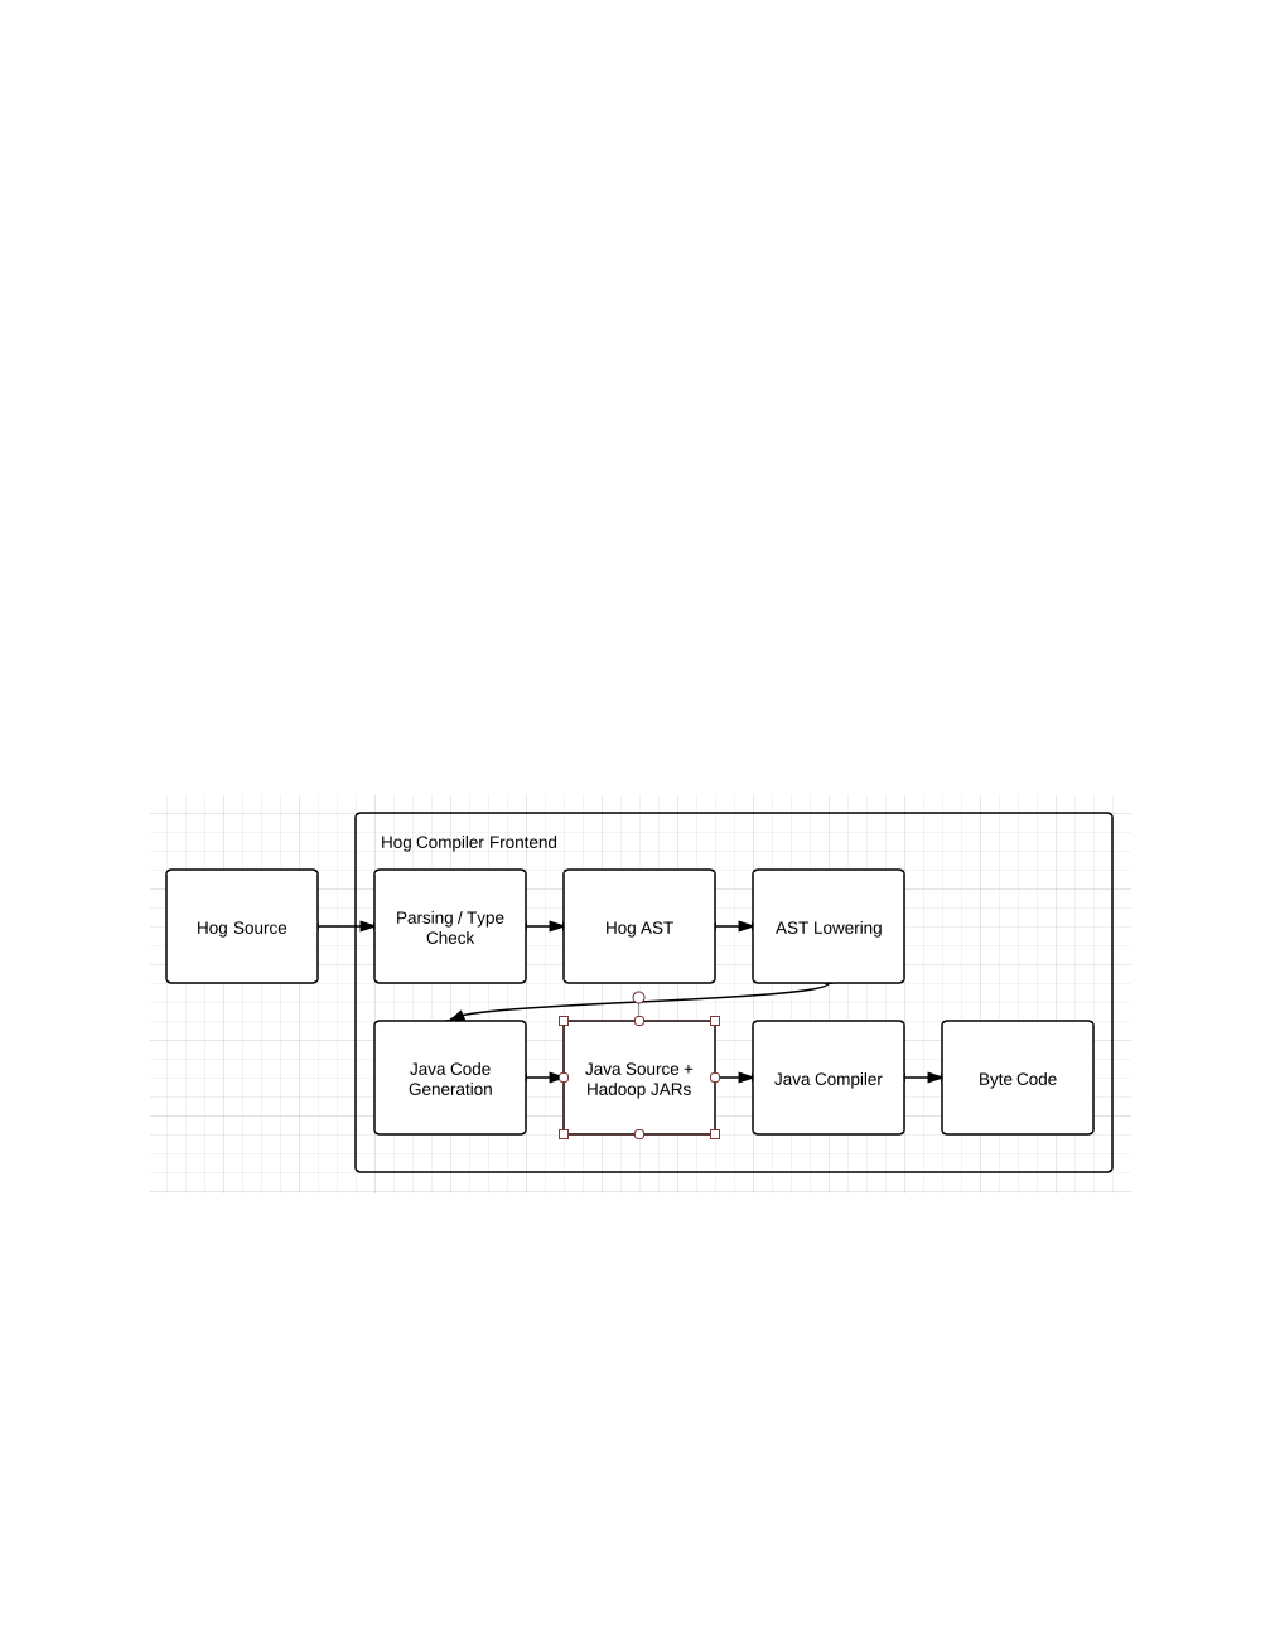
\includegraphics[width=1.0\textwidth]{img/hog_compiler.pdf}
  \caption{The overall structure of the Hog compiler.}
\end{figure}
\end{center}

\subsection{Usage} % (fold)
\label{sub:usage}

% subsection usage (end)

To build and run a Hog source file there is an executable script \tt hog
\rm that automates the compilation and linking steps for the user. \\

Usage: \tt hog [--hdfs|--local] job <job args> \rm
\begin{itemize}
  \item[] \tt --hdfs\rm: if job ends in '.hog' or '.java' and the file exists, link it against the hadoop JARFILE and then run it on HOST.
  \item[] \tt --local\rm: run on local host.
\end{itemize}

\subsection{Example} % (fold)
\label{sub:example}

\begin{verbatim}
hog --local WordCountJob.hog --input someInputFile.txt --output ./someOutputFile.csv
\end{verbatim}

This runs the \tt wordCount \rm job in \emph{local} mode (i.e. not on a Hadoop
cluster).

% subsection example (end)

% section linkage_and_i_o (end)

\section{Exception Handling} % (fold)
\label{sec:exception_handling}

Similar to some other programming languages (such as Java and C++), Hog uses an
exception model in which an exception is thrown and can be caught by a catch
block. Code should be surrounded by a try block and then any exceptions
occurring within the try block will subsequently be caught by the catch block.
Each try block should be associated with at least one catch block. However,
there can be multiple catch blocks to handle specific types of exceptions. In
addition, an optional finally block can be added. The finally block will
execute in all circumstances, whether or not an exception is thrown. The
structure of exception handling should be similar to this, although there can
be multiple catch blocks and the finally block is optional:

\begin{quotation}
\tt try \{ \rm \\
\indent \indent \emph{expression;} \\
\tt \indent \} catch ( \rm \emph{exception} \tt ) \rm \{ \\
\indent \indent \emph{expression;} \\
\tt \indent \} finally \rm \{ \\
\indent \indent \emph{expression;} \\
\tt \indent \}
\end{quotation}

The current version of the language does not support the programmer throwing
exceptions, only catching them.

Because the proper behavior of a Hog program is dependent on resources outside of
the language (i.e. the proper behavior of the user’s Hadoop software), there are
more sources exceptions in Hog than most general purpose languages. These sources
can be divided into two categories: \textbf{\emph{compile­-time exceptions}} and
\textbf{\emph{internal run­-time exceptions}}.

\subsection{Compile-time Errors} % (fold)
\label{sub:compile_time_exceptions}

The primary cause of most compile-­time exceptions in Hog are semantic errors. Such
errors are unrecoverable because it is impossible for the compiler to properly
interpret the user program. Some compilers for other languages offer a limited
amount of compile-­time error correction. Because Hog programs are often designed
to process gigabytes or terabytes of data at a time, the standard Hog compiler
offers no compile-­time error correction. The assumption is that a user would
rather re­tool their program than risk the chance of discovering, only after hours
of processing, that the compilers has incorrectly assumed what the user meant. The
following are Hog compile-­time exceptions:

\begin{itemize}
  
  \item[] \tt FunctionNotDefinedError \rm
  
   Thrown when a program attempts to carry out an operations of the sort \tt
variable.builtInFunction() \rm where \tt variable \rm is some variable and \tt
builtInFunction \rm is a built-in function, and either \tt builtInFunction \rm
cannot operate on variables of that type or \tt builtInFunction \rm  is not
defined as a built-in function.
  
  \item[] \tt InvalidFunctionArgumentsError \rm
   
    Thrown when a program calls a function with the wrong number or type of
parameters. For example, if we define the function \tt max(int a, int b) \rm,
this error will be thrown if the program contains a construct like \tt
max(2,3,4) \rm or \tt max("hello", 3) \rm.

   \item[] \tt TypeMismatchError \rm  

   Thrown when a program attempts to carry out an operation on a variable of
the wrong type (like adding a \tt text \rm and an \tt int \rm together).
  
   \item[] \tt UnreachableCodeError \rm

   Thrown when code is included in a part of a program that will never be
executed (e.g. code after a return statement that can never be reached).

\end{itemize}

% subsection compile_time_exceptions (end)

\subsection{Internal Run-time Exceptions} % (fold)
\label{sub:internal_run_time_exceptions}

Internal run­time exceptions include such problems as I/O exceptions (i.e. a
specified file is not found on either the user’s local file system or the
associated Hadoop file system), type mismatch exceptions (i.e. a program
attempts to place two elements of different types into the same list) and
parsing exceptions. The following are Hog internal run-­time exceptions:


\begin{itemize}
  \item[] \tt FileNotFoundException \rm
  
  Thrown when the the Hog program attempts to open a non-existent file.
  
  \item[] \tt FileLoadException \rm
  
  Thrown when an error occurs while Hog is attempting to read a file (e.g. the
file is deleted while reading).
  
  \item[] \tt ArrayOutOfBoundsException \rm
  
  Thrown when a program tries to access a non-valid index of a \tt list\rm.
  
  \item[] \tt IncorrectArgumentException \rm
  
  Thrown when a derived-type object is instantiated with invalid parameters, or
a function is called with invalid parameters.
  
  \item[] \tt TypeMismatchException \rm
  
  Thrown when a program attempts to carry out an operation on a variable of the
wrong type (like adding a \tt text \rm and an \tt int \rm together).
    
  \item[] \tt NullReferenceException \rm
  
  Thrown whenever the value of a variable cannot be \tt null \rm (e.g. in \tt
myList.get(i)\rm, if \tt i \rm is \tt null\rm, the operation with throw a \tt
NullPointerException\rm).
  
  \item[] \tt ArithmeticException \rm
  
  Thrown whenever an arithmetic operation is attempted on non-numeric operands.
  
\end{itemize}

% section internal_run_time_exceptions (end)

% section exception_handling (end)

\section{Grammar} % (fold)
\label{sec:grammar}

\emph{Note}: The presented grammar has one minor ambiguity relating to the
\textbf{\emph{dangling-else}} problem. If the grammar is run through the parser
generator \tt yacc\rm, \tt yacc \rm will identify 7 shift/reduce parsing-action
conflicts. However, the ambiguity is handled by the default behavior of \tt
yacc\rm, which preferences shift to reduce, associating \tt else \rm and \tt
elseif \rm clauses with the closest \tt if \rm clause.


\begin{verbatim}
terminal DECR, INCR, RETURN, CONTINUE;
terminal TIMES, DIVIDE, MOD;
terminal LESS, GRTR, LESS_EQL, GRTR_EQL, DBL_EQLS, NOT_EQLS, ASSIGN;
terminal TEXT, BOOL, INT, REAL, VOID;
terminal MINUS, UMINUS, PLUS;
terminal ARROW, DOT;
terminal String TEXT_LITERAL;
terminal String ID;
terminal String INT_CONST;
terminal String REAL_CONST;
terminal String BOOL_CONST;
terminal String CASE;
terminal BREAK, DEFAULT;
terminal AND, OR, NOT;
terminal WHILE, FOR, FOREACH, IN, IF, ELSE, ELSEIF, SWITCH;
terminal FUNCTIONS, MAIN, MAP, REDUCE;
terminal L_BRACE, R_BRACE, L_BRKT, R_BRKT, L_PAREN, R_PAREN, SEMICOL, COL, COMMA;
terminal LIST, ITER, SET;
terminal TRY, CATCH, FINALLY;
terminal ExceptionTypeNode EXCEPTION;

nonterminal GuardingStatementNode GuardingStatement;
nonterminal CatchesNode Catches;
nonterminal IdNode CatchHeader;
nonterminal StatementListNode Finally;
nonterminal StatementListNode Block;
nonterminal StatementListNode ExpressionStatements;
nonterminal ExpressionNode ForExpr;
nonterminal StatementListNode ForInit;
nonterminal StatementListNode ForIncr;
nonterminal DerivedTypeNode DictType;

nonterminal ProgramNode Program;
nonterminal SectionNode Functions;
nonterminal SectionNode Main;
nonterminal SectionNode Map;
nonterminal SectionNode Reduce;
nonterminal SectionTypeNode SectionType;
nonterminal StatementNode Statement;
nonterminal ExpressionNode ExpressionStatement;
nonterminal StatementNode FunctionList;
nonterminal StatementNode IterationStatement;
nonterminal StatementNode LabeledStatement;
nonterminal SelectionStatementNode SelectionStatement;
nonterminal StatementNode DeclarationStatement;
nonterminal StatementListNode StatementList;
nonterminal ElseIfStatementNode ElseIfStatement;
nonterminal ElseStatementNode ElseStatement;
nonterminal JumpStatementNode JumpStatement;
nonterminal ExpressionNode EqualityExpression;
nonterminal ExpressionNode LogicalExpression;
nonterminal ExpressionNode LogicalTerm;
nonterminal ExpressionNode RelationalExpression;
nonterminal ExpressionNode Expression;
nonterminal ExpressionNode AdditiveExpression;
nonterminal ExpressionNode MultiplicativeExpression;
nonterminal ExpressionNode CastExpression;
nonterminal ExpressionNode UnaryExpression;
nonterminal ExpressionNode PostfixExpression;
nonterminal ExpressionNode PrimaryExpression;
nonterminal ExpressionNode Constant;
nonterminal ExpressionNode ArgumentExpressionList;
nonterminal FunctionNode Function;
nonterminal ParametersNode ParameterList;
nonterminal TypeNode Type;
nonterminal UnOpNode.OpType UnaryOperator;
nonterminal Types.Derived DerivedType;

precedence left MINUS, PLUS;
precedence right UMINUS;
precedence right ELSE;
precedence right ELSEIF;
precedence right L_PAREN;

start with Program;

Program::=
    Functions Map Reduce Main
  ;

Functions::=
    FUNCTIONS L_BRACE FunctionList R_BRACE
  |
    /* epsilon */
  ; 
 
FunctionList::=
    Function
  |
    FunctionList Function
  ;

Function::=
    Type ID L_PAREN ParameterList R_PAREN L_BRACE StatementList R_BRACE
  ;

ParameterList::=
    ParameterList COMMA Type ID
  |
    Type ID
  |
    /* epsilon */
  ;

Map::=
    MAP SectionType L_BRACE StatementList R_BRACE
  ;

Reduce::=
    REDUCE SectionType L_BRACE StatementList R_BRACE
  ;

SectionType::=
    L_PAREN Type ID COMMA Type ID R_PAREN ARROW L_PAREN Type COMMA Type R_PAREN
  ;

Main::=
    MAIN L_BRACE StatementList R_BRACE
  ;

StatementList::=
    Statement
  |
    StatementList Statement
  ;

Statement::=
    ExpressionStatement
  |
    SelectionStatement
  |
    IterationStatement
  |
    LabeledStatement
  |
    JumpStatement
  | 
    DeclarationStatement
  | 
    GuardingStatement
  | 
    Block
  ;

GuardingStatement::=
     TRY Block Finally
   |
     TRY Block Catches
   | 
     TRY Block Catches Finally
   ;

Block::=
    L_BRACE StatementList R_BRACE
  | 
    L_BRACE R_BRACE
  ;

Finally::=
    FINALLY Block
  ;

Catches::=
     CatchHeader Block
   | 
     Catches CatchHeader Block
   ;

CatchHeader::=
     CATCH L_PAREN EXCEPTION ID R_PAREN
   ;
 
DeclarationStatement::=
    Type ID
  |
    Type ID ASSIGN Expression
  ;
 
JumpStatement::=
    CONTINUE
  |
    BREAK
  |
    RETURN ExpressionStatement
  ;
 
ExpressionStatement::=
    SEMICOL
  |
    Expression SEMICOL
  ;

Expression::=
    LogicalExpression
  |
    UnaryExpression ASSIGN Expression
  ;

LogicalExpression::=
    LogicalExpression OR LogicalTerm
  |
    LogicalTerm
  ;

LogicalTerm::=
    LogicalTerm AND EqualityExpression
  |
    EqualityExpression
  ;

EqualityExpression::=
    RelationalExpression
  |
    EqualityExpression DBL_EQLS RelationalExpression
  |
    EqualityExpression NOT_EQLS RelationalExpression
  ;

RelationalExpression::=
    AdditiveExpression
  |
    RelationalExpression LESS AdditiveExpression
  |
    RelationalExpression GRTR AdditiveExpression
  |
    RelationalExpression LESS_EQL AdditiveExpression
  |
    RelationalExpression GRTR_EQL AdditiveExpression
  ;

AdditiveExpression::=
    MultiplicativeExpression
  |
    AdditiveExpression PLUS MultiplicativeExpression
  |
    AdditiveExpression MINUS MultiplicativeExpression
  ;

MultiplicativeExpression::=
    CastExpression
  |
    MultiplicativeExpression TIMES CastExpression
  |
    MultiplicativeExpression DIVIDE CastExpression
  |
    MultiplicativeExpression MOD CastExpression
  ;

CastExpression::=
    UnaryExpression
  |
    L_PAREN Type R_PAREN CastExpression
  ;

UnaryExpression::=
    UnaryOperator CastExpression
  |
    PostfixExpression
  ;
  
UnaryOperator::=
    MINUS 
    %prec UMINUS
  |
    NOT
  ;

PostfixExpression::=
    PrimaryExpression
  |
    ID DOT ID
  |
    ID DOT ID L_PAREN ArgumentExpressionList R_PAREN
  |
    ID L_PAREN ArgumentExpressionList R_PAREN
  |
    PostfixExpression INCR
  |
    PostfixExpression DECR
  ;

ArgumentExpressionList::=
    Expression
  |
    ArgumentExpressionList COMMA Expression
  |
    /* epsilon */
  ;

PrimaryExpression::=
    ID
  |
    Constant
  |
    L_PAREN Expression R_PAREN
  ;

Constant::=
    INT_CONST
  |
    REAL_CONST
  |
    BOOL_CONST
  |
    TEXT_LITERAL
  ;

SelectionStatement::=
    IF Expression Block ElseIfStatement ElseStatement
  |
    SWITCH Expression L_BRACE StatementList R_BRACE
  ;

ElseIfStatement::=
    ELSEIF Expression Block ElseIfStatement
  |
    /* epsilon */
  ;

ElseStatement::=
    ELSE Block
  |
    /* epsilon */
  ;

IterationStatement::=
    WHILE L_PAREN Expression R_PAREN Block
  |
    FOR L_PAREN ForInit ForExpr ForIncr R_PAREN Block
  |
    FOR L_PAREN ForInit ForExpr R_PAREN Block
  |
    FOREACH Type ID IN Expression Block
  ;

ForInit::=
    ExpressionStatements
  |
    DeclarationStatement SEMICOL
  ;

ForExpr::=
    ExpressionStatement
  ;

ForIncr::=
    ExpressionStatements
  ;

ExpressionStatements::=
    ExpressionStatement
  |
    ExpressionStatements COMMA ExpressionStatement
  ;
 
LabeledStatement::=
    CASE LogicalExpression COL Statement
  |
    DEFAULT COL Statement
  ;

Type::=
    VOID
  |
    TEXT
  |
    BOOL
  |
    INT
  |
    REAL
  |
    DerivedType:d LESS Type:t GRTR
  ;

DerivedType::=
    LIST
  |
    ITER
  |
    SET
  ;

\end{verbatim}

\chapter{Project Plan}
\label{chap:plan}

Written by Samuel Messing (sbm2158).

\section{Development Process}

The scope of the Hog programming language was ambitious from the start. Our
stated goal was to create a general-purpose scripting language which made
carrying out distributed computation simple and intuitive. As such, from the
beginning we were interested in ways to make the implementation of the language
as simple as possible. The following goals were identified early on:

\begin{itemize}
\item make the build system as simple as possible,
\item make the logic of our individual modules as similar as possible,
\item document everything,
\item use a distributed version control system,
\item write verbose and informative log statements.
\end{itemize}

Focusing on these goals throughout the development enabled use to work concurrently
on different aspects of the compiler and maintain a codebase that was both readable
and easy to understand.  

\subsection{Simplicity of Build System}

As project manager, I worked early on with both the System Architect (Ben) and
the System Integrator (Kurry) to come up with a build system that was simple and
easily extensible. After trying a few different options, we decided on Ant,
a build system similar to Make, specialized for the Java programming language.
Another advantage of going with Ant is that both JFlex and Cup, the frameworks
we used to construct the lexer and parser, respectively, have native Ant support.
Identifying and implementing our build system early on enabled us to move quickly
and write code that we were sure worked across all of our machines. 

\subsection{Similarity of Modules}

Throughout the project, I worked very closely with the System Architect (Ben) to
develop and build common data structures that could be used across all of our
code. The abstract syntax tree was made in a generic enough way so that all
of our different tree walks could use the exact same tree class, without having
to support and debug different implementations of the same interface or abstract
parent class.  

Personally, I also developed our Types class, which was a static class that
contained several convenience methods for handling types across the entirety
of the compiler. These methods include type checking, type conversion and
as well as additional functionality required for internal functionality. I
set out to write the class as early as possible so that both elements of
the frontend and the backend could make use of it. Simplifying and unifying how
different modules handled the same information enabled everyone on the team to
read each other's code qand quickly understand how it functioned.

\subsection{Document Everything}

One of the most undersold parts of Java is it's well thought out documentation
schema (JavaDocs). Early on I realized that in order for us to be able to work
semi-independently on different modules we would need to have a robust set of
documentation. By using JavaDoc instead of regular comments, we were able to
generate HTML documentation, which more clearly provides an overview of the entire
architecture of our compiler, and allowed everyone on our team to work quickly and
respond to updated classes appropriately.

One of the largest challeneges in this project was developing a set of node classes
for our abstract syntax trees that captured the right granularity of information,
without beeing too complex that handling corner cases became intractable. Our
System Architect (Ben) found a great tool that generated UML diagrams for our
class hierarchies, which in concert with our JavaDocs helped to make development
as simple and efficient as possible. 

\subsection{Distributed Version Control}

As soon as our team was formed I created a git repository on
Github.com\footnote{\texttt{http://www.github.com/smessing/Hog}} for use by the
team. One of the first things we discussed as a team was what workflow pattern
we wanted to use throughout the course of the project. Very quickly we decided
on a continuous-build pattern, where the main branch of our git repository 
(master) was reserved for compiling, tested, and finalized code. Any classes
that were currently in development existed in separate branches, and were only
merged into master after sufficient amount of testing. Each programmer maintained
their own branch for development. If two or more programmers were working on the
same class, a new, shared branch was created. By being conservative about what
code was merged into the master branch, we were able to work independently, without
fear that someone else's work would be interrupted by leaving our individual code
in an unfinished state. 

\subsection{Verbose Logging}

Another advantage of programming in Java is the robust and sophisticated logging
libraries available to the programmer. Around the same time that the build system
was developed, the System Architect (Ben) investigated several different logging
libraries and wrote a tutorial for the rest of us on how to use it. The logging
library supported several levels of log statements, FINEST, FINER, FINE, INFO,
WARNING and SEVERE (from most verbose to least). We decided that FINEST and FINER
were to be used strictly for debugging, while FINE was to be used to document 
normal behavior, at a level of detail that was concise enough for all developers
to look at, but still too verbose for the user. INFO, WARNING and SEVERE were
reserved for statements that the user would see. By identifying and keeping
to these log levels early on, we were able to quickly identify bugs and 
inefficient or errant behavior. 

\section{Roles and Responsibilities}

\begin{itemize}
\item Ben, System Architect 
\begin{quotation}
\noindent Ben's major responsibilities included developing the fundamental data structures
used by the compiler, working out the different elements of the compiler and
how they interrelate, and developing the symbol table.   
\end{quotation}
\item Jason, Testing/Validation
\begin{quotation}
\noindent Jason's major responsibilities included testing all of the elements of our compiler,
and working on the aspects of the compiler related to type checking, and developing
the symbol table.
\end{quotation}
\item Kurry, System Integrator
\begin{quotation}
\noindent Kurry's major responsibilties included developing a clean interface between
Hog and Hadoop and working on the Hog wrapper program that builds, compiles and
runs Hog source programs.  
\end{quotation}
\item Paul, Language Guru
\begin{quotation}
\noindent Paul's major responsibility was determining the syntax and semantics of our
language, and developing the semantic analyzer.
\end{quotation}
\item Sam, Project Manager
\begin{quotation}
\noindent As project manager, my major responsibilities included setting project deadlines,
assigning work, and making sure that we met our goals. I was also responsible
for developing the classes to translate Hog programs into Java programs. 
\end{quotation}
\end{itemize}

\section{Hog's Developer Style Sheet}

We made use of the standard Java style guide, including such conventions as camel
case, verbs for functions and method names, and hierachical object classes. For
formatting, we used Eclipse's auto-format feature to keep our code looking as
consistent as possible. 

\section{Project Timeline}

\begin{itemize}
\item[] January
\begin{quotation}
\noindent Developed several potential ideas for languages. Met with Aho and decided on
implementing Hog, a MapReduce language.   
\end{quotation}
\item[] February
\begin{quotation}
\noindent Worked on the White Paper for our language, developed both the goals of our language
and the overall ``feel'' (simple, minimal boilerplate code, easy-to-read syntax).
Started to sketch out overall compiler architecture, and decided on frameworks
(JFlex for the lexer, CUP for parser, Hadoop framework for executing distributed computation, and Java as target language) and development environments (Eclipse, Git, Github, \LaTeX $\,$ for documentation). 
\end{quotation}
\item[] March
\begin{quotation}
\noindent Wrote the language reference manual and tutorial for our language. 
Developed the build system (Ant for compiling compiler code, Make for running
the compiler on Hog source programs), implemented and tested the parser and lexer,
and developed the fundamental data structures (abstract syntax tree, node classes).
\end{quotation}
\item[] April
\begin{quotation}
\noindent Implemented tree walking algorithms to populate the symbol table, perform
type checking, perform semantic analysis and generate Java source code. Wrote
tests for the walkers. 
\end{quotation}
\item[] May
\begin{quotation}
\noindent Refactored code and worked on documentation. Developed more tests and
worked on fixing bugs. 
\end{quotation}
\end{itemize}

\section{Project Log}

\begin{itemize}
\item[] January
\begin{itemize}
\item[] Week of January 22nd
\begin{itemize}
\item Met to discuss language ideas.
\end{itemize}
\item[] Week of January 29th
\begin{itemize}
\item Decided on Hog, and Java as implementation language.
\end{itemize}
\end{itemize}
\item[] February
\begin{itemize}
\item[] Week of Feburary 5th
\begin{itemize}
\item Decided on Hadoop as the framework for executing distributed computation.
\item Decided on JFlex framework for implementing the lexer.
\item Decided on CUP framework for implementing the parser. 
\end{itemize}
\item[] Week of February 12th
\begin{itemize}
\item Discussed and figured out development environment (Java, Ant, Eclipse, Git).
\item Started working on white paper.
\end{itemize}
\item[] Week of February 19th
\begin{itemize}
\item Started git repository.
\item Finished white paper.
\end{itemize}
\item[] Week of February 26th 
\begin{itemize}
\item Began the language reference manual (LRM). 
\end{itemize}
\end{itemize}
\item[] March
\begin{itemize}
\item[] Week of March 4th
\begin{itemize}
\item Started Eclipse project.
\item Worked on LRM and tutorial.
\end{itemize} % march 4th
\item[] Week of March 11th
\begin{itemize}
\item Began developing the Hog grammar.
\item Worked on LRM and tutorial.
\item Started working on wrapper program functionality (program that runs the
Hog compiler to compile source programs).
\end{itemize} % march 11th
\item[] Week of March 18th
\begin{itemize}
\item Finished the Hog grammar.
\item Finished the tutorial and LRM.
\item Began developing the lexer.
\end{itemize}
\item[] Week of March 25th
\begin{itemize}
\item Took the week off to study for the midterm.
\end{itemize}
\end{itemize} % march
\item[] April
\begin{itemize}
\item[] Week of April 1st
\begin{itemize}
\item Worked on the lexer.
\item Started developing the abstract syntax tree and node classes.
\item Started developing the parser.
\item Implemented developer build system.
\end{itemize} 
\item[] Week of April 8th
\begin{itemize}
\item Developed ConsoleLexer class for development and testing of lexer. 
\item Developed lexer JUnit tests. 
\item Finished abstract syntax tree, including iterators for post- and pre-order 
traversals.
\item Developed mock classes for testing.
\end{itemize}
\item[] Week of April 15th
\begin{itemize}
\item Further development/refinement of node classes.
\item Developed more semantic actions for parser, mainly to construct node classes.
\item Parsed our first program! 
\end{itemize}
\item[] Week of April 22nd
\begin{itemize}
\item Developed/implemented basic type functionality.
\item Further refinement of the grammar.
\item Implemented logging details. 
\item Refinement of node classes and ASTs.
\item Started tree walking algorithms (identified the visitor pattern as our
common design pattern for tree walks).
\item Begain developing symbol table class.
\end{itemize}
\item[] Week of April 29th
\begin{itemize}
\item Finished implementation of symbol table class.
\item Finished type checking / symbol table population walks.
\item Implemented java source generator.
\item Implemented tests for walkers and parser. 
\item Finished compiler.
\end{itemize}
\end{itemize} % april
\end{itemize} % log


\chapter{Language Evolution}
\label{chap:evo}

\begin{itemize}
\item Describe how the language evolved during the implementation and what steps were used to try to maintain the good attributes of the original language proposal.
\item Describe the compiler tools used to create the compiler components.
\item Describe what unusual libraries are used in the compiler.
\item Describe what steps were taken to keep the LRM and the compiler consistent.
\end{itemize}

The initial intent was to make Hog stylistically and aesthetically resemble Python. In our first discussions about the language, we had envisioned statements being separated by line breaks and dynamic typing.

\chapter{Translator Architecture}
\label{chap:trans}

To be written by Ben.

\begin{itemize}
\item Show the architectural block diagram of translator.
\item Describe the interfaces between the modules.
\item State which modules were written by which team members.
\end{itemize}

\chapter{Development and Run-Time Environment}
\label{chap:environ}

To be written by Kurry.

\begin{itemize}
\item Describe the software development environment used to create the compiler.
\item Show the makefile used to create and test the compiler during development.
\item Describe the run-time environment for the compiler.
\end{itemize}

\chapter{Test Plan}
\label{chap:test}

As the tester and validator for Team Hog, I set out to create a systematic, automated set of tests at each step in the process of building a compiler. In order to make sure that each part of the design worked according to our specification, I tried to include tests that touched as many aspects of the language as possible. 

I considered each of the testing phases to be a two-step process. First, create a basic set of tests with the assumption that the compiler worked as expected. These tests would touch a variety of areas of the language. These were our black box tests because they were built without the need to know what was going on under the hood. Then, the second step of the process was to attempt to break the language in as many ways as possible. These tests required an intimate knowledge of the nuances of the language and were therefore our white box tests. I tried to incorporate as many boundary cases as possible into these tests. At each phase of the testing, we uncovered various bugs and unimplemented aspects of the language that we fixed on subsequent iterations. I will briefly touch upon each phase of testing and the challenges and outcomes faced throughout the process. All of these tests are in the ‘test’ package in our source code. The tests were developed using Java’s JUnit development framework.

\subsection*{Lexer Testing (\tt LexerTester.java\rm)}
 
In order to test the lexical analysis of Hog programs, I created a large variety of short code snippets, passed them to the lexer and made sure that the correct tokens were being returned. For example, when the string ``a++`` was passed to the lexer, I created tests with \tt assertEquals()\rm to make sure that the first token returned was ID and the second token returned was INCR. I started with small tests that only touched two to five token streams and built towards strings that were thirty tokens long. This phase helped us discover certain tokens that were not being returned correctly and needed to be added/modified in the lexer, such as \tt TEXT\rm, \tt TEXT\_LITERAL\rm, and \tt UMINUS\rm. A sample lexer test can be seen at the end of this section.

\subsection*{Parser Testing (\tt ParserTester.java\rm)}

This was the most challenging aspect of the testing process. Due to the limitation of built-in parsing methods, it was difficult to create an automated set of tests for the parser that tested each part of the grammar. This phase relied more heavily on manual testing than I would have preferred. We were able to run a variety of programs through the parser and focused on breaking the parser and touching as many edge cases as possible. This allowed us to uncover the bugs and produce code that was not correctly parsed. We had to modify and expand the grammar from the results of this testing. The tests that we created for the parser were the motivation for creating such specific node subclasses that captured the different details associated with each production. In addition, information that we gathered in testing the parser also allowed us to create a clean design for the symbol table, which is constructed during parsing and the first walk of our AST.

\subsection*{Symbol Table Testing (\tt SymbolTableTester.java\rm)}
I found when I reached this phase of creating tests that there were certain details of the node classes that I needed to gain a better understanding of in order to write tests. For this reason, I worked closely with Ben and Paul in designing and implementing the Symbol Table and worked with Ben on the Symbol Table Visitor and Type Checking Visitor. In order to test the construction of the Symbol Table, we created several sample programs, created the Symbol Table from these programs and analyzed the symbol table to make sure the information was being correctly captured. In addition, we also made sure reserved words and functions were in the reserved symbol table at the root of the Symbol Table structure. There were two key issues related to creating nested scopes that were uncovered during testing and an important issue related to adding function parameters and argument lists to the symbol table. This phase also focused on making sure the correct exceptions were being thrown – i.e. VariableRedefinedException, VariableUndeclaredException, etc.

\subsection*{Abstract Syntax Tree Testing (\tt AbstractSyntaxTreeTester.java\rm)}

In order to test the AST, we created an automated set of tests that was based on the pre and post order traversals of the AST. First, we created an AST during the set up phase of the testing and made sure that we included a variety of node structures on the tree. Then, we did both a preorder walk of the tree and a postorder walk of the tree and made sure the traversals were occurring in the correct order.  

\subsection*{Type Checking Testing (\tt TypesTester.java\rm \,and \tt  TypeCheckingTester.java\rm)}

During this walk of the AST, we did type checking and decorated the tree with the correct types. I created many of the tests for this part of the design as Ben and I implemented functionality in the type check walk. The first part of type checking testing was to make sure the functions that we wrote around type compatibility were operating correctly. For example, we had to make sure if we visit a BiOpNode with the plus operator that the operands are both text (concatenation) or numbers (addition). Once the tests proved that these functions were all valid, we moved to implementing tests on the walk of an actual AST to make sure type decorating was occurring according to our rules. This part of the testing uncovered the fact that our IdNodes were not being decorated at all during our initial walk, so we added the functionality to the TypeCheckingVisitor to handle this.  

\subsection*{Code Generation Testing (\tt CodeGeneratingTester.java\rm)}

The goal for the code generation tests was to determine whether or not our programs were being correctly mapped to Hadoop programs written in Java. These tests focused on using the code generating visitor walk of the tree to make sure that the structure, meaning and types of our Hog programs were being captured during the transformation to Java. Besides writing tests, this step of the testing involved actually running the Hadoop programs on our local machines and on Amazon Elastic MapReduce to see if the programs would run without errors and if the results in the output files were in line with what we expected.

\subsection*{Testing Hog Programs}

In order to prepare us for testing, I set us up on Amazon Web Services to run our programs on Amazon’s Elastic MapReduce platform. We upload the jar of our compiled program and the input files to Amazon’s S3 storage platform, then we launch the Elastic MapReduce job on a small cluster with 2 instances. The output files are stored in S3 after the processing has successfully completed. The instructions for running a Hog program on AWS are detailed in the report.

For several aspects of our implementation, we focused on a pair approach to programming and to testing. Since Sam handled a lot of the implementation regarding lexical analysis and parsing, he also worked with me to create additional tests for these phases to make sure we captured everything. In addition, he also added type tests for some additional type functions that he wrote. Kurry created some tests for the node structure since he also worked on creating ASTs. In addition, since I wanted to really understand the node structure, symbol table and visitor pattern, I worked together with Ben and Paul in designing and implementing the symbol table, designing the visitor pattern for Hog and implementing the Type Checking walk. Working on these aspects of the project enabled me to write better tests since I had a deeper understanding of these classes. I also think that writing tests helped Kurry and Sam better understand the aspects of the project that they were working on. 

One of the main challenges during testing was capturing the breadth and depth of the Hog language in all of the tests. Testing, in conjunction with development, was an iterative process that required us to add and modify the testing suites as functionality was added to and removed from the language specification. As the tester and validator for this project, I believe I have developed the skills to more rigorously test software. More importantly, I learned a lot about the principles related to strong software design and software engineering during the entire process. 

\subsection*{Sample Test from \tt LexerTester.java\rm}

\begin{verbatim}
/**
* Tests for correct parsing of the postfix increment operator
* 
* Specifically, ensures that Lexer produces a token stream of ID * INCR 
*     for strings like "a++"
* 
* @throws IOException

	@Test
	public void incrementSymbolTest() throws IOException {

		String text = "a++";
		StringReader stringReader = new StringReader(text);
		Lexer lexer = new Lexer(stringReader);
		List<Integer> tokenList = new ArrayList<Integer>();
		Symbol token = lexer.next_token();

		while (token.sym != sym.EOF) {
			tokenList.add(token.sym);
			token = lexer.next_token();
		}

		assertEquals(
"It should produce 2 tokens for the string '" + text + "'", 2, tokenList.size());
assertEquals("The first token should be a ID", sym.ID, tokenList.get(0)
				.intValue());
assertEquals("The second token should be a INCR", 
               sym.INCR, tokenList.get(1).intValue());
	}
\end{verbatim}

\chapter{Conclusions}
\label{chap:concl}

\section{Lessons Learned}
\label{sec:lessons}



\subsection{Jason's Lessons}
\label{sub:jasons-lessons}

To be written by Jason.

\subsection{Sam's Lessons}
\label{sub:sams-lessons}

To be written by Sam.

\subsection{Ben's Lessons}
\label{sub:bens-lessons}

To be written by Ben.

\subsection{Kurry's Lessons}
\label{sub:kurrys-lessons}

I think the most important lesson learned was about how to make good judgments
on what our language should support and should not support, and I think that
came from a lot of bad judgements we made early on about what we were going to
support in our language. Our language was by far much more sophisticated than the
other languages made by the class, but we also had to cut some things out of our
language just because we did not have the man power or time frame necessary to
implement them. 

From a project planning standpoint, I think that the team should have all worked 
together on building the abstract syntax tree and node classes, instead of making
that work modular in the beginning. This is due to the fact that all parts of the team
rely at using a working abstract syntax tree, and if the AST is not complete early on
in the project, it make creating the other parts of the compiler very difficult. 



\subsection{Paul's Lessons}
\label{sub:pauls-lessons}

To be written by Paul.

\section{Advice for Other Teams}

Don't take this class.

\section{Suggestions for Instructor}

Things we'd like to see more of:

\begin{itemize}
\item More details  
\item More discussion of functional languages
\end{itemize}

\appendix

\chapter{Code Listing}

\begin{itemize}
\item \texttt{back\_end} package
\begin{enumerate}
\item \texttt{CodeGenerationVisitor.java}
\begin{quotation}
\noindent An AST-walker that translates Hog programs into Java programs. Written by Samuel Messing.
\end{quotation}
\item \texttt{ErrorCheckingVisitor.java}
\begin{quotation}
\noindent An AST-walker that performs semantic analysis. Written by Paul Tylkin.
\end{quotation}
\item \texttt{SymbolTableVisitor.java}
\begin{quotation}
\noindent An AST-walker that populates symbol tables. Written by Benjamin Rapaport and Jason Halpern.
\end{quotation}
\item \texttt{TypeCheckingVisitor.java}
\begin{quotation}
\noindent An AST-walker that performs basic type checking and type inference. Written by Jason Halpern and Benjamin Rapaport. 
\end{quotation}
\item \texttt{Visitor.java}
\begin{quotation}
\noindent The abstract class that all visitors inherit, specifies the behavior of the Visitor design pattern. Written by Jason Halpern.
\end{quotation}
\end{enumerate} % end back_end package
\item \texttt{front\_end} package
\begin{enumerate}
\item \texttt{ConsoleLexer.java}
\begin{quotation}
\noindent 
\end{quotation}
\item \texttt{Hog.java}
\begin{quotation}
\noindent 
\end{quotation}
\item \texttt{Lexer.java}
\begin{quotation}
\noindent 
\end{quotation}
\item \texttt{Parser.java}
\begin{quotation}
\noindent 
\end{quotation}
\item \texttt{sym.java}
\begin{quotation}
\noindent 
\end{quotation}
\item \texttt{Lexer.jflex}
\begin{quotation}
\noindent 
\end{quotation}
\item \texttt{Parser.cup} 
\end{enumerate} % end front_end package
\item \texttt{test} package
\begin{enumerate}
\item \texttt{AbstractSyntaxTreeTester.java}
\begin{quotation}
\noindent 
\end{quotation}
\item \texttt{CodeGeneratingTester.java}
\begin{quotation}
\noindent 
\end{quotation}
\item \texttt{LexerTester.java}
\begin{quotation}
\noindent 
\end{quotation}
\item \texttt{NodeTester.java}
\begin{quotation}
\noindent 
\end{quotation}
\item \texttt{SymbolTableTester.java}
\begin{quotation}
\noindent 
\end{quotation}
\item \texttt{TypeCheckingTester.java}
\begin{quotation}
\noindent 
\end{quotation}
\item \texttt{TypesTester.java}
\begin{quotation}
\noindent 
\end{quotation}
\end{enumerate} % end test package
\item \texttt{util.ast} package
\begin{enumerate}
\item \texttt{AbstractSyntaxTree.java}
\begin{quotation}
\noindent 
\end{quotation}
\item \texttt{TreeTraversalBuilder.java}
\begin{quotation}
\noindent 
\end{quotation}
\end{enumerate} % end util.ast package
\item \texttt{util.ast.node} package
\begin{enumerate}
\item \texttt{ArgumentsNode.java}
\begin{quotation}
\noindent 
\end{quotation}
\item \texttt{BiOpNode.java}
\begin{quotation}
\noindent 
\end{quotation}
\item \texttt{CatchesNode.java}
\begin{quotation}
\noindent 
\end{quotation}
\item \texttt{ConstantNode.java}
\begin{quotation}
\noindent 
\end{quotation}
\item \texttt{DerivedTypeNode.java}
\begin{quotation}
\noindent 
\end{quotation}
\item \texttt{ElseIfStatementNode.java}
\begin{quotation}
\noindent 
\end{quotation}
\item \texttt{ElseStatementNode.java}
\begin{quotation}
\noindent 
\end{quotation}
\item \texttt{ExceptionTypeNode.java}
\begin{quotation}
\noindent 
\end{quotation}
\item \texttt{ExpressionNode.java}
\begin{quotation}
\noindent 
\end{quotation}
\item \texttt{FunctionNode.java}
\begin{quotation}
\noindent 
\end{quotation}
\item \texttt{GuardingStatmenetNode.java}
\begin{quotation}
\noindent 
\end{quotation}
\item \texttt{IdNode.java}
\begin{quotation}
\noindent 
\end{quotation}
\item \texttt{IfElseStatementNode.java}
\begin{quotation}
\noindent 
\end{quotation}
\item \texttt{IterationStatementNode.java}
\begin{quotation}
\noindent 
\end{quotation}
\item \texttt{JumpStatementNode.java}
\begin{quotation}
\noindent 
\end{quotation}
\item \texttt{MockExpressionNode.java}
\begin{quotation}
\noindent 
\end{quotation}
\item \texttt{MockNode.java}
\begin{quotation}
\noindent 
\end{quotation}
\item \texttt{Node.java}
\begin{quotation}
\noindent 
\end{quotation}
\item \texttt{ParametersNode.java}
\begin{quotation}
\noindent 
\end{quotation}
\item \texttt{PostfixExpressionNode.java}
\begin{quotation}
\noindent 
\end{quotation}
\item \texttt{PrimaryExpressionNode.java}
\begin{quotation}
\noindent 
\end{quotation}
\item \texttt{PrimitiveTypeNode.java}
\begin{quotation}
\noindent 
\end{quotation}

\item \texttt{ProgramNode.java}
\begin{quotation}
\noindent 
\end{quotation}
\item \texttt{RelationalExpressionNode.java}
\begin{quotation}
\noindent 
\end{quotation}
\item \texttt{ReservedWordTypeNode.java}
\begin{quotation}
\noindent 
\end{quotation}
\item \texttt{SectionNode.java}
\begin{quotation}
\noindent 
\end{quotation}
\item \texttt{SectionTypeNode.java}
\begin{quotation}
\noindent 
\end{quotation}
\item \texttt{SelectionStatementNode.java}
\begin{quotation}
\noindent 
\end{quotation}
\item \texttt{StatementListNode.java}
\begin{quotation}
\noindent 
\end{quotation}
\item \texttt{StatementNode.java}
\begin{quotation}
\noindent 
\end{quotation}
\item \texttt{SwitchStatementNode.java}
\begin{quotation}
\noindent 
\end{quotation}
\item \texttt{TypeNode.java}
\begin{quotation}
\noindent 
\end{quotation}
\item \texttt{UnOpNode.java}
\begin{quotation}
\noindent 
\end{quotation}
\end{enumerate} % end util.ast.node
\item \texttt{util.error} package
\begin{enumerate}
\item \texttt{FunctionNotDefinedError.java}
\begin{quotation}
\noindent 
\end{quotation}
\item \texttt{InvalidFunctionArgumentError.java}
\begin{quotation}
\noindent 
\end{quotation}
\item \texttt{MissingReturnError.java}
\begin{quotation}
\noindent 
\end{quotation}
\item \texttt{TypeMismatchError.java}
\begin{quotation}
\noindent 
\end{quotation}
\item \texttt{UnreachableCodeError.java}
\begin{quotation}
\noindent 
\end{quotation}
\item \texttt{VariableRedefinedError.java}
\begin{quotation}
\noindent 
\end{quotation}
\item \texttt{VariableUndeclaredError.java}
\begin{quotation}
\noindent 
\end{quotation}
\end{enumerate} % end util.error
\item \texttt{util.logging} package
\begin{enumerate}
\item \texttt{BreifLogFormatter.java}
\begin{quotation}
\noindent 
\end{quotation}
\end{enumerate} % end util.logging
\item \texttt{util.symbol\_table} package
\begin{enumerate}
\item \texttt{FunctionSymbol.java}
\begin{quotation}
\noindent 
\end{quotation}
\item \texttt{Method.java}
\begin{quotation}
\noindent 
\end{quotation}
\item \texttt{ReservedSymTable.java}
\begin{quotation}
\noindent 
\end{quotation}
\item \texttt{ReservedWordSymbol.java}
\begin{quotation}
\noindent 
\end{quotation}
\item \texttt{Symbol.java}
\begin{quotation}
\noindent 
\end{quotation}
\item \texttt{SymbolTable.java}
\begin{quotation}
\noindent 
\end{quotation}
\item \texttt{VariableSymbol.java}
\begin{quotation}
\noindent 
\end{quotation}
\item \texttt{Word.java}
\begin{quotation}
\noindent 
\end{quotation}
\end{enumerate} % end util.symbol_table
\item \texttt{util.type} package
\begin{enumerate}
\item \texttt{Types.java}
\begin{quotation}
\noindent 
\end{quotation}
\end{enumerate}
\end{itemize}  % end total

Include a listing of the complete source code with identification of who wrote
which module of the compiler. This listing does not have to be included in the
paper copy of the final report.

\nocite{*}
\bibliographystyle{acm}
\bibliography{references}

\end{document}
